
\chapter{Experimental infrastructure}
\markboth{\thechapter. EXPERIMENTAL INFRASTRUCTURE}{}
\label{chap:apparatus}
	\begin{adjustwidth}{0cm}{0cm}
	\begin{flushright}
	\singlespacing
	\emph{``Every sensor is a temperature sensor.\\
	 Some sensors measure other things too."\\} 
	- Engineer's aphorism\footnote{Quoted without attribution in Elecia White's \emph{Making Embedded Systems}, O'Reilly media (2011).}
	\end{flushright}
	\end{adjustwidth}
	\onehalfspacing
	\vspace{1cm}
	{While} nature abhors a vacuum, experimentalists abhor a background.
	Ultracold atom experiments require ultra-high vacuum (UHV) conditions because collisions with a background gas can easily overcome the frail forces that hold the atoms in their traps.
	% H F Hess, Evaporative cooling of magnetically trapped and compressed spin-oolarized hydrogen, Physical Review B 34, 3476-3479, Sept 1986
	% W Ketterle and N J van Druten, Evaporative cooling of traped atoms, advanes in atomic molecular and optical physics 37, 181-236, 1996
	% O J Luiten, M W reynolds, J T M Walraven, Kinetic theory of the evaporative cooling of a trappe dgas, Physical Reveiw A 53, 381-389 Jan 1996s works conducted on two experimental apparatus built around the skeletal structure of their respective vacuum systems.
	The major works discussed in chapters \ref{chap:transitions},  \ref{chap:tuneout} and \ref{chap:QD} were undertaken on a machine which has been in productive operation for many years\footnote{This machine is described in great detail in past publications \cite{Swansson04,Dall07_BEC} and PhD dissertations \cite{HodgmanThesis,ManningThesis,ShinThesis,DallThesis}.
	This chapter presents a summary description. The motivated reader is referred to the aforementioned sources for more information, and to the texts \cite{FootAtomic,MetVdS} for general information about cooling and trapping techniques.}.
	This machine achieved BEC in 2007 \cite{Dall07_BEC}, utilizing a bright cold beam of helium \cite{Swansson04} and optimized Zeeman slower \cite{Dedman04}.
	Key technical facilitations were the installation of auxiliary field coils for active cancellation of stray magnetic fields \cite{Dedman04}, and ambient air temperature control to the centikelvin level at the BEC chamber by control of the cooling air mixture \cite{Dedman15}.
	The machine has had a storied history since then, hosting a range of experimental themes including testing quantum-electrodynamic predictions of electronic transition rates \cite{Dall08}, momentum correlations between many atoms \cite{Hodgman17,Dall13,Manning13} (especially Hanbury Brown-Twiss correlations \cite{Manning10,Dall11a,Hodgman11,Rugway11,Rugway13}), studies of atom lasers \cite{Dall07_laser,Dall08a,Henson18_BCR,Manning10} and guided matter waves \cite{Dall10, Dall11a,Dall11}, and quantum-optics demonstrations such as single-particle sources \cite{Manning14}, ghost-imaging \cite{Khakimov16,Hodgman19}, and foundational topics such as Wheeler's delayed choice thought experiment \cite{Manning15}, and Bell-type correlations between pairs of freely propagating atoms \cite{Shin19}.
	This machine was also used for proof-of-principle demonstrations of a machine-learning assisted optimization of a quantum transport protocol \cite{Henson18_ML} and 3D magnetic gradiometry with pairs of atoms \cite{Shin20}.
	While I was a collaborator on the latter two works, they are not included in this thesis.
	My main work on this machine include laser spectroscopic measurements of several transition energies \cite{Ross20,Thomas20} (the former constituting chapter \ref{chap:transitions}); a measurement of the 413 nm tune-out wavelength (as first reported in \cite{Henson15} and improved during the course of this thesis, discussed in Chapter \ref{chap:tuneout}); and measurement of the quantum depletion of a condensate as described in chapter \ref{chap:QD}.
	

	About half the duration of this course of study was devoted to the refurbishment of a retired cold-atom experiment towards loading a \mhe~BEC into an optical lattice.
	The two machines can be distinguished by their intended final trapping method: The first-described machine can therefore be called the \emph{BiQUIC machine}, and the upgraded apparatus referred to as the \emph{lattice machine}.
	Before its erstwhile retirement, the lattice machine was used for the study of electron scattering and  dual-species MOT experiments \cite{Uhlmann05,Byron10,Byron10a} and determination of electronic transition rates in \mhe~\cite{Hodgman09_23P} .
	The renovation of the lattice machine was motivated by the insufficient optical access into the BEC chamber of the BiQUIC machine, preventing a straightforward upgrade to incorporate several additional trapping beams.
	BEC was recently achieved in the lattice machine by the resident graduate students \cite{Abbas21}, and the construction is ongoing.
	As the lattice machine has yet to produce scientific results in its newfound youth, I will discuss the scientific motivation for its construction and my contributions to the project in appendix \ref{chap:lattice}.
	The present chapter is concerned with the anatomy of the BiQUIC machine, which hosted the works described in chapters \ref{chap:transitions}, \ref{chap:tuneout}, and \ref{chap:QD}.

\section{Helium beamline}

\subsection{Vacuum system}
	Our vacuum is maintained by continuous operation of several turbomolecular pumps\footnote{One of the earliest accomplishments of significant vacuum was by Lavoisier, who used pumps from the fire station to evacuate a chamber.
	Since then vacuum has advanced considerably, and at ultrahigh vacuum the exhaust is so dilute that one does not have the viscosity to operate pumps in the true sense.
	Nonetheless, the name remains.}, backed by roughing pumps that vent directly to the atmosphere.
	For the UHV chambers where BEC is created, an additional turbomolecular pump operates between the vacuum-adjacent turbo and the roughing pump.
	
	The vacuum systems form the skeleton of both machines, which have a common structure illustrated schematically in Figs. \ref{fig:apparatus} \& \ref{fig:apparatus_2}.


	

	The placement of some of the turbomolecular pumps, Faraday cups, and pressure gauges differ between the machines, but this makes no functional difference.
	However, the beamline of the lattice machine does not feature a deflection stage or a focusing stage for the \emph{low-velocity intense source} of helium (LVIS).
	The BiQUIC machine has more limited optical access and has featured the addition of a tunable titanium-sapphire laser (section \ref{sec:spec_laser}).
	A major difference between the two setups is the configuration of the chamber that houses the final trapping stage where BEC is achieved (which is still under development in the lattice machine).
	Otherwise, the overall structure of the vacuum systems is the same and so only the BiQUIC machine is shown in its entirety in in Figs. \ref{fig:apparatus} \& \ref{fig:apparatus_2}.
	For comparison, the apparatus around the lattice machine's science chamber is shown and described in appendix \ref{chap:lattice}.

	% 	\begin{figure}
	% 	\centering
	% 	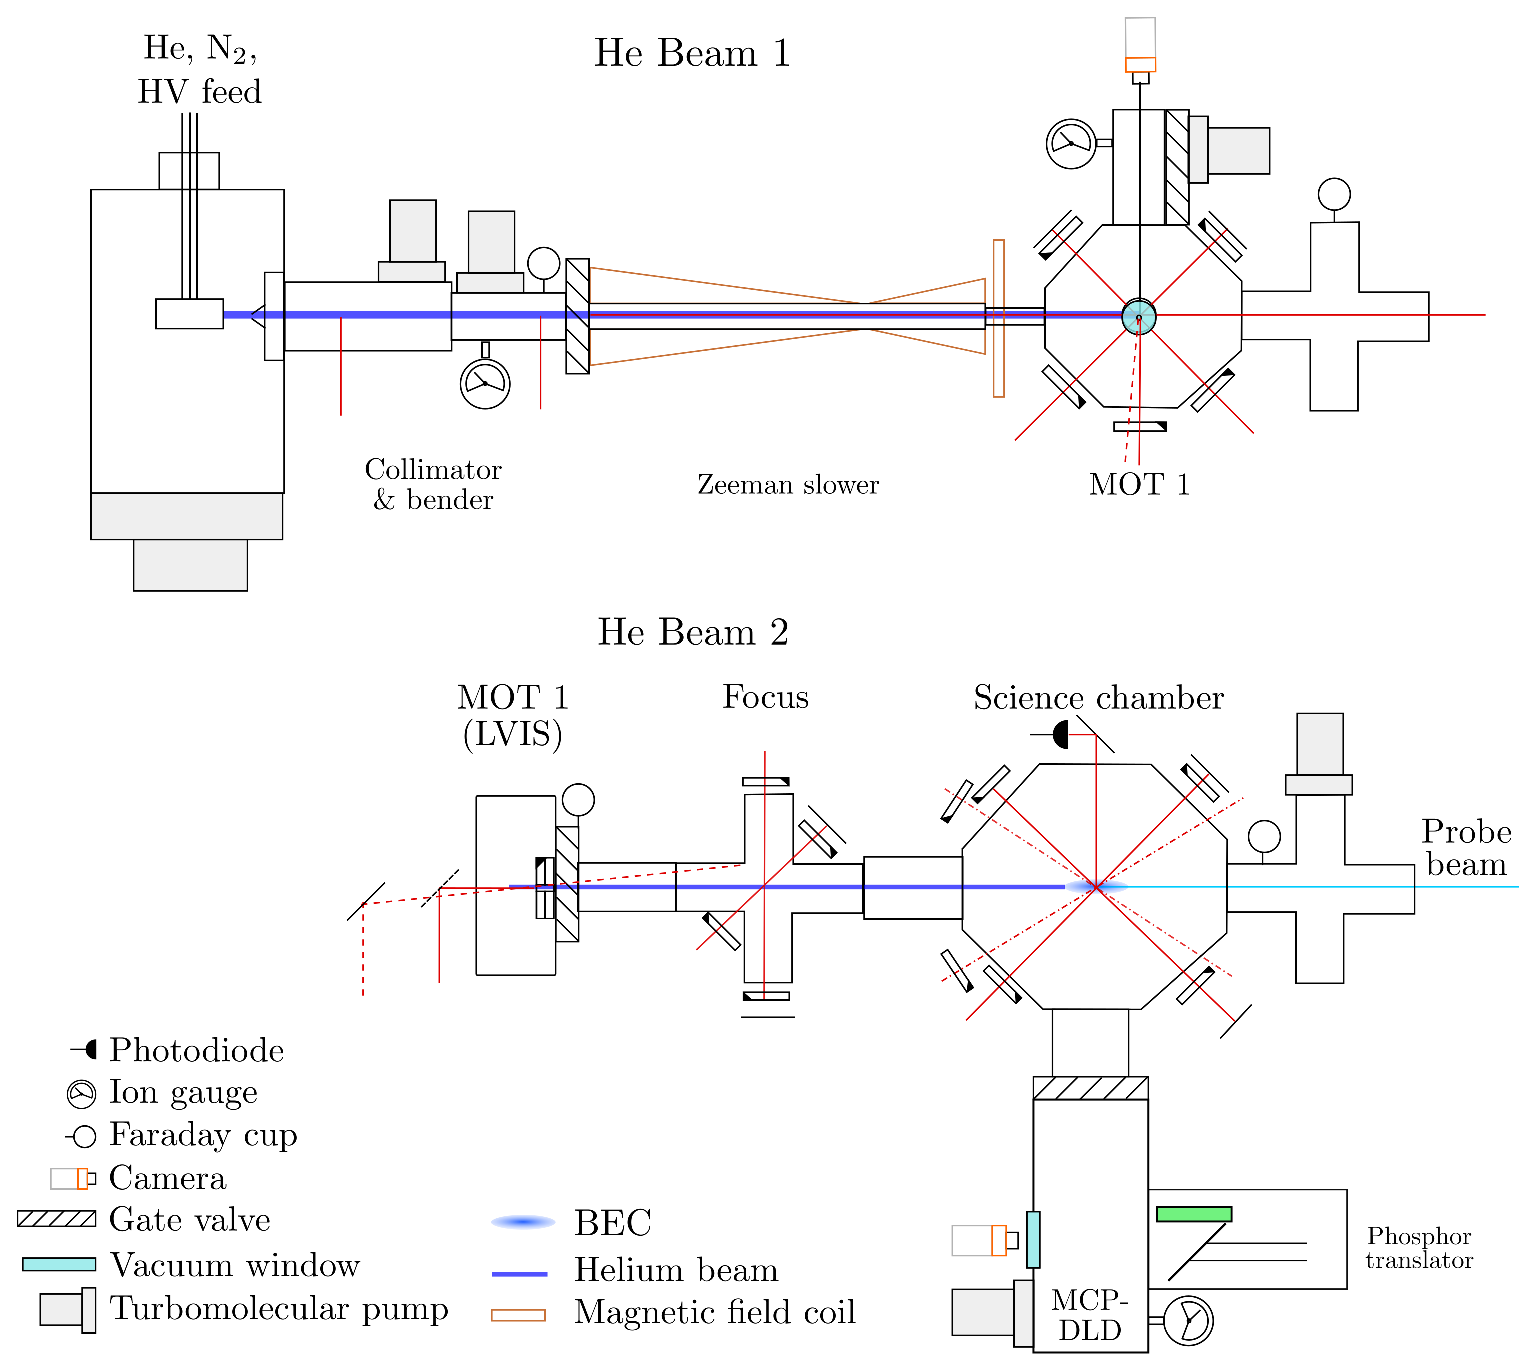
\includegraphics[width=\textwidth]{fig/apparatus/vacuum_schematic_simplified}
	% 	\caption{Vacuum system and laser insertion optics used in the BiQUIC machine.  The following features are not present in the lattice mahine: The spectroscopic laser (blue line) is inserted through a vacuum window along the weak ($x$) axis of the trap.  A phosphor-screen-backed MCP (green) is mounted above a 45$^\circ$ mirror permitting imaging of the phosphor pattern with a camera. This is typically used for troubleshooting and alignment rather than scientific purposes, and so is moved out of the fall-line with an in-vacuum translation mount.}
	% 	\label{fig:apparatus}
	% \end{figure}

	\begin{figure}
		\centering
		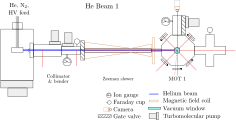
\includegraphics[width=\textwidth]{fig/apparatus/vacuum_schematic_split_1}
		\caption{Vacuum system and laser insertion optics for initial cooling of the helium from room temperature to the mK scale in the first MOT. The helium source is cooled by liquid $\textrm{N}_2$ and sustained by a high-voltage (HV) DC discharge.
		Cooling and trapping beams (solid red lines) are transmitted via free-space links from the AOM table and inserted through flange-mounted windows.
		The collimation and bending stage provide intial cooling and background reduction before feeding into the Zeeman slower, which reduces the longitudinal velocity of the atoms so they can be captured by the first MOT at the end of beam 1. 
		The horizontal beam in the first MOT is retro-reflected though a quarter-wave plate mounted on a mirror with a 2 mm hole bored through the centre, which feeds cold helium from MOT 1 into science chamber (see Fig. \ref{fig:apparatus_2})}
		\label{fig:apparatus}
	\end{figure}

	\begin{figure}
		\centering
		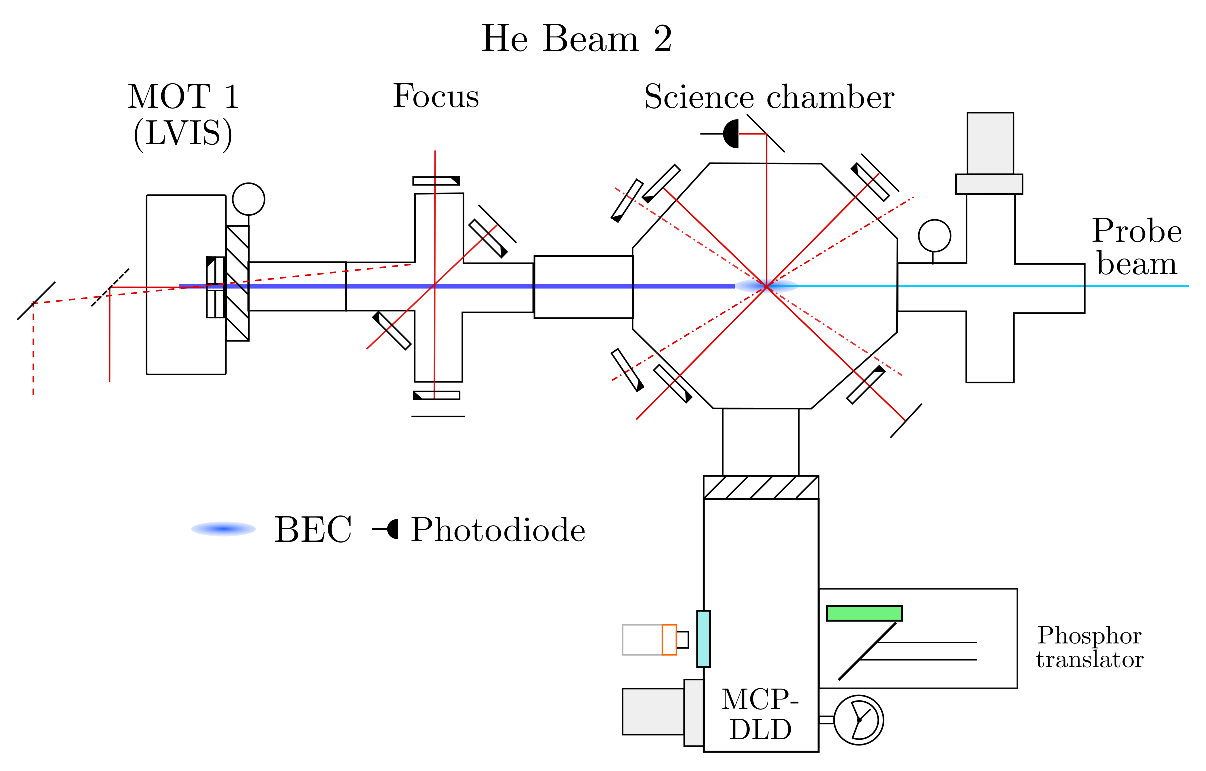
\includegraphics[width=\textwidth]{fig/apparatus/vacuum_schematic_split_2}
		\caption{Schematic of the second beamline. The low-velocity intense source (LVIS) of \mhe~ atoms is formed by kicking atoms from the first MOT into the ultra-high vacuum conditions of the science chamber with a slightly blue-detuned `push' beam. Doppler cooling beams (red dot-dash lines) lower the temperature before commencing evaporative cooling. Two other features are present in this diagram, and abesnt in the lattice machine. The spectroscopic laser (blue line) is inserted through a vacuum window along the weak ($x$) axis of the trap. A phosphor-screen-backed MCP (green) is mounted above a 45$^\circ$ mirror permitting imaging of the phosphor pattern with a camera. This is typically used for troubleshooting and alignment rather than scientific purposes, and so is moved out of the fall-line with an in-vacuum translation mount. }
		\label{fig:apparatus_2}
	\end{figure}
	

\subsection*{\mhe~atom source}

	The metastable \mhe~state is generally produced by a DC electric discharge as opposed to optical excitation due to the lack of convenient X-ray light sources at 63 nm.
	Electrons accelerated by a strong potential gradient can ionize helium atoms, and thus also have enough energy to excite atoms into the \mhe~state (or achieve it by recombination and/or relaxation along a decay pathway including the $\MetastableState$ state).
	In our experiments, a grounded copper block cooled by liquid nitrogen serves as the anode and reaction vessel.
	A tungsten cathode is held at 2 kV and placed in front of the vessel, separated by electrically insulating boron nitride spacers.
	The breakdown voltage of helium gas in this geometry is lowest at a pressure above the standard operating setting, and even then an additional 2.5 kV pulse is required to achieve ignition before turning the source pressure down into the operating regime.
	Unfortunately, the DC discharge only excites about .01\% of the atoms into the \mhe~state \cite{Stas06}.
	Further, the light mass of helium means that even at temperatures around 70 K (thanks to the liquid nitrogen cooling) the atoms have fairly high velocities necessitating a Zeeman slower stage before the initial trapping stage. 
	The source chamber tends to operate consistently over a year or so, permitting development and execution of a handful of experimental campaigns.
	However, the copper housing degrades with use.
	The first symptom of an ailing source is intermittent extinctions and, if not promptly addressed, an inability to successfully strike.
	This is remedied by extracting the source chamber from the vacuum system and skimming a few microns of material from the interior surface of the block, a procedure which is  straightforward but painstaking.
	

\subsection*{Beam forming}

	The gas expands out of the forward-facing aperture of the reaction vessel and a small solid angle is selected by a skimming nozzle between the source chamber and the rest of the helium beamline.
	The skimmer also functions as a differential pumping stage by rejecting atoms with large transverse velocities, and keeping the first laser cooling stages at a lower pressure than the source chamber.
	The \mhe beam is collimated by a single laser beam reflected in a figure-4 configuration, forming a a 2D optical molasses \cite{Lett81,Rooijakkers96} and providing cooling in the two transverse degrees of freedom.
	Before insertion into the chamber, a cylindrical lens expands the laser beam into an ellipse with a roughly 5:1 aspect ratio. The long axis is parallel to the helium beamline. 
	This extends the interaction zone to about 10 cm. 
	The beams are offset in the image plane here for clarity, but in reality they are offset along the axis of the helium beam.
	In the schematic, the beam passes through the four-way intersection of the laser beams. 
	The laser detuning (red of resonance) ensures that only atoms moving against the laser propagation are Doppler-shifted towards resonance, hence reducing the beam divergence.
	% \footnote{Technically speaking, the beam is not collimated in the same manner as a laser beam.
	% The divergence is reduced, but not eliminated such that the spot size remains fixed or becomes focused.}.
	% \begin{wrapfigure}{l}{0.5\textwidth}
	% \begin{figure}
	% 	\centering
	% 	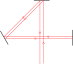
\includegraphics[width=0.5\textwidth]{fig/apparatus/figure_4_beams}
	% 	\caption{Schematic of the figure-4 configuration used for transverse cooling of the source beam in the collimation stage. }
	% 	\label{fig:figure_4}
	% \end{figure}


	This is followed by a `bending' stage wherein a single laser beam, picked off from the collimator beam, deflects the metastable atoms by a few degrees through a second stage of differential pumping, which blocks the line of sight from the source to the MOT, into the Zeeman slower chamber.
	This provides better selectivity of \mhe~atoms by reducing the number of unexcited atoms that enter the Zeeman slower and first MOT chamber.
	% \subsection*{Optical molasses}
	% P D Lett, W D Phillips, S L Rolston, CE Tanner, R N Watts, C I Wetbrook, Optical Molasses, journal of the optical society of america B 6, 2084-2107, Nov 1981
	% W Rooijakkers, Wo Hogervorst, W Vassen, an intense collimated beam of metastable helium atoms by two-dimensional laser cooling, Optics COmmunications 123, january 1996

	Zeeman slowers, so named for the exploitation of the Zeeman effect\footnote{In the earier days of cold atom science they were sometimes called \emph{Zeeman-compensated slowers} \cite{Mastwijk98}}, are necessary to slow atoms from thermal characteristic of their sources to below the capture velocity of the magneto-optical traps located at the end of the slower.
	An atom moving with respect to a laser source (as described in section \ref{sec:doppler_basics}) in a magnetic field $\textbf{B} = B\hat{b}$ will have its electronic resonances shifted by the Doppler and Zeeman effects, which can be summarized as
	\begin{equation}
		\omega_{0,\text{lab}} = \omega_{0}\left(1 + \frac{k\cdot v}{c}\right) + \frac{\mu_B B}{\hbar}\left(g_e m_e - g_g m_g\right),
	\end{equation}
	where the $g$-factors and magnetic quantum numbers $m$ of the ground and excited state are denoted by $g$ and $e$, respectively. 
	Hence, a carefully architected magnetic field can compensate for the changing Doppler shift as atoms decelerate.
	The $\sigma^+$ light employed in our Zeeman slower drives the cooling transition with $g_g m_g = 2\times 1$ and $g_e m_e = \frac{3}{2}\times2$, leading to a field-dependent shift of $\approx1.4$ MHz/G.
	
	The magnetic field profile for maximum deceleration depends on the initial velocity, and so the spread of initial velocities according to the Maxwell-Boltzmann distribution necessitates another figure of merit to optimize against.
	In our experiments the Zeeman slower coil windings are built to create a field profile that maximizes the number of atoms slowed below the capture velocity of the first MOT \cite{Dedman04}.
	The Zeeman slower thus reduces the most probable longitudinal velocity of the beam from $\approx700$ m/s to $\approx70$ m/s, which permits loading of the MOT to a steady-state population in about one second.

	% W Rooijakkers, Wo Hogervorst, W Vassen, an intense collimated beam of metastable helium atoms by two-dimensional laser cooling, Optics COmmunications 123, january 1996

\subsection*{First Magneto-Optical Trap}
	% cooper94 temperature of atoms in a MOT
	The magneto-optical trap combines the radiation pressure with a spatially-varying magnetic field to confine atoms in three dimensions.
	Current-carrying coils in an anti-Helmholtz configuration create a locally linear magnetic strength (about the zero in the centre) with a gradient of the form $(B',B',-2B')$ where the stronger gradient is along the axis of symmetry. 
	Because the Zeeman shift of the levels in the helium $2\triplet S_1$ and $2\triplet P_2$ manifold are linear functions of the magnetic field strength (at least in regimes relevant to our traps, where the fine structure splitting of the $2\triplet P$ states is a thousandfold larger than the Zeeman shift), the cooling transition exhibits a Zeeman shift which is proportional to the distance from the centre of the trap.
	We drive the $\sigma^+$ transition between the $2\triplet S_1(m_J=1)$ and $2\triplet P_2(m_J=2)$ states, and red-detune the laser to ensure the light is resonant on an ellipsoidal shell around the trap centre.
	The atoms also exhibit a Doppler broadening from their motion within the trap, but this amounts to a broadening of $\approx100$ kHz at $\approx1$ mK, which is tiny in comparison with the $\approx 100$ MHz ($\approx 70\Gamma$) shift in the $1.6$ MHz-wide transition, a small correction to the picure just outlined\footnote{The Maxwellian distribution of velocities in a thermal cloud leads to a broadening of the absorption line due to the range of Doppler shifts experienced by the atoms. The Doppler-broadened linewidth can be calculated through $\Delta_{D} = \sqrt{8 k_B T\log(2)/(mc^2)}\omega_0$, where $\Delta$ is the broadened linewidth and $\omega_0$ is the resonant frequency \cite{FootAtomic}.}.
	The net result is that as an atom moves away from the origin of the trap, the probability of it absorbing a photon from the beam pointing back towards the origin increases, thus creating a restoring force along each axis.

	This technique was first proposed by Jean Dalibard and eventually realised by Raab \emph{et al} \cite{Raab87}.
	The population of early helium MOTs were limited because the small size of the trap and low detunings led to high densities and thus rapid deterioration by Penning losses.
	Later attempts achieved larger atom numbers by operating with larger beams and detunings (-22$\Gamma$), obtaining lower densities than in other species and mitigating losses due to Penning ionization \cite{Tol99}.
	The multifaceted physics of MOTs has proven rich ground for study in general \cite{Townsend95,Walker90}, and also in the specific case of helium, for which the two-body loss rate has been studied \cite{Tol99} along with the roles of light-assisted collisions \cite{Stas06,McNamara07}. 
	Temperatures in a MOT are, at best, on the order of the steady-state molasses temperature $\approx1$ mK \cite{Lett81}.
	Further evaporative cooling is therefore required to reach quantum degeneracy.
	
	The background pressure in the first MOT chamber is still too high to maintain a long-lived magnetic trap.
	Therefore, the first MOT is used as a source for a secondary helium beam which feeds into the science chamber.
	The MOT chamber features a $\approx$2 mm hole bored through a compound quarter-waveplate-and-mirror mounted inside the vacuum chamber (see Figs. \ref{fig:apparatus} \& \ref{fig:apparatus_2}), which adjoins the transfer conduit supplying the BEC chamber with cold helium.

	A slightly blue-detuned `push' beam is used to kick atoms through the aperture at the back of the first MOT into the second MOT along ballistic trajectories \cite{Swansson04}.
	In practise the beam points slightly upward, and the orientation is optimized by maximizing the saturated fluorescence signal in the second MOT (see section \ref{sec:he_detection}for a description of the technique).
	The atoms pass through a `focus' stage consisting of two crossed, retro-reflected laser beams with a $\approx$1 cm waist.
	Wire coils mounted around the (horizontal) 2$\frac{3}{4}$" window flanges create a quadrupole magnetic field surrounding the beamline such that the circularly-polarized beams address only atoms on the half of the beam proximal to the optical insertion.
	This final stage of transverse cooling increases the efficiency of loading the second MOT from the \mhe~beam.
	The focusing stage typically increases the saturated fluorescence signal in the second MOT by at least 50\%.
	

\subsection*{The Science Chamber}

	The second trapping chamber is evacuated to a pressure of some $10^{-11}$ mbar, yielding an excellent magnetic trap lifetime (permitting optical interrogation periods of up to 25 seconds after the $\approx$20 second BEC production sequence in one recent measurement \cite{Thomas20}).
	The chamber is surrounded by three pairs of square magnetic coils which actuate active cancellation of stray fields from the earth and nearby electronic equipment\footnote{The `nuller' reduces, but does not eliminate, 50Hz noise from the AC mains supply to the laboratory.} \cite{Dedman07}.
	This assists the creation of a stable magnetic trap with two coil pairs in a Bi-planar quadrupole Ioffe configuration (BiQUIC) \cite{Dall07}.
	These coils also generate the field which maintains the second MOT, wherein the final stage of optical cooling is provided by a pair of low-intensity Doppler cooling beams inserted at 15$^\circ$ relative to the horizontal \cite{Dall07_BEC}.
	The transfer between the two traps is achieved by simply switching off the light.


	Magnetic traps exploit the interaction between the atomic magnetic dipole and a magnetic field, taking the form $E_B = -\mu\cdot \textbf{B} = -\hbar g m_J B$.
	A magnetic field with a local extremum can therefore form a confining potential for the states whose energy is minimized at this point.
	It follows from the Earnshaw's theorem that a magnetic field in free space cannot have any local maxima \cite{Harms00,MakingProbingUnderstanding}, and so one must select an atomic state with $g m_J>0$ for confinement at a local minimum of the magnetic field strength.
	In \mhe~this uniquely selects the $m_J=+1$ state for magnetic trapping, which also ensures complete spin-polarization and the attendant reduction in Penning losses.
	The BiQUIC design is a solution to a critical issue with early traps \cite{Migdall85}: The quadrupole fields generated by coils in an anti-Helmholtz configuration feature a zero crossing in the trap centre.
	Atoms in a magnetic field undergo transitions to untrapped states, known as \emph{Majorana transitions}, at a rate proportional to $\exp(-B/\omega)$, where $\omega$ is the trapping frequency and $B$ is the magnitude of a (uniform) magnetic field \cite{Sukumar97}.
	In harmonic traps the Zeeman splitting at the trap minimum thus sets the upper bound on the Majorana transition rate \cite{Brink06}.
	Many variations on the quadrupole trap exist to mitigate this issue, including the Time-Orbiting Potential (TOP) \cite{Petrich95}, Ioffe-Pritchard \cite{Pritchard83}, cloverleaf \cite{Mewes96}, and QUIC \cite{Esslinger98} traps, while other groups have added a repulsive dipole potential to the trap zero with a focused and blue-detuned laser beam \cite{Davis95}.
	The magnetic trap enables forced evaporative cooling to below the condensation threshold, some three orders of magnitude colder than the limits of optical cooling. 


  

	\begin{figure}
	\begin{minipage}{0.55\textwidth} %4-8-16
	\vspace{0pt}
		\includegraphics[width=\textwidth]{fig/apparatus/biquic_coil.pdf}

	\end{minipage}
	\hfill
	\begin{minipage}{0.45\textwidth}
	\vspace{0pt}
	\caption{Schematic diagram of the Bi-QUIC coil design. Black arrows indicate the direction of current flow. The cylindrical coordinate axes indicate the axis of symmetry ($z$), which has a lower trapping frequency than the 'tight' axes. In this thesis, the experiments typically use traps with a `weak' axis with frequency $\omega_z\approx55$ Hz and `tight' axis with frequency $\omega_\perp\approx 430$ Hz. Diagram reproduced with permission from \cite{Dall07}}
	\end{minipage}
	\end{figure}

	A comprehensive introduction to evaporative cooling can be found in \cite{Ketterle96}; see \cite{FootAtomic,PethickSmith} for more compact discussions. 
	Here I present a short, intuitive picture of evaporative cooling in a semiclassical, non-interacting model. 
	A gas of bosons at finite temperature will consist of atoms whose energies are described by Bose-Einstein statistics (see chapter \ref{chap:theory}). 
	At equilibrium, the expected population of single-particle states falls off exponentially with energy $E$. 
	Therefore there will be some atoms which have much greater energy than the average. 
	If these atoms are confined in a magnetic trap, then the more energetic atoms will be more likely to be found further from the trap origin.
	The wavefunction of the high-energy atoms will thus be supported in regions with larger magnetic fields than the lower-energy atoms.
	Therefore it is possible to selectively remove the high-energy atoms by driving the transition between trapped and untrapped states with radio-frequency (RF) radiation tuned to the resonance near the Zeeman splitting seen by only the most energetic atoms in the trap.
	After a timescale on the order of a few times the (inverse) inter-atomic collision rate, the gas rethermalizes (i.e. regains the Bose-Einstein statistics after having its tail cut off) at a lower temperature by virtue of losing its most energetic constituents.
	Repeating this process for lower RF frequencies removes atoms with progressively lower energies, cooling the sample.
	If one ramps the radio frequency down too quickly, then the loss rate of atoms can counteract the loss of temperature and result in a decrease in phase-space density, i.e. moving further from the condensation threshold.
	Conversely, a ramp that is slow will be more efficient but also more subject to other trap loss channels and needlessly prolong the experimental cycle.
	Theoretically optimal evaporative cooling ramps are discussed in \cite{Ketterle96}, and in practise we apply a continuous RF sweep from 20 MHz down to $\approx800$ kHz, with an empirically-optimized and roughly exponential shape over about 20 seconds.
	The endpoint of the ramp depends on the configuration of the BiQUIC trap (specifically the trapping frequency and the bias at the trap centre) and the desired size and temperature of the condensate. 
	


	Two radio antennas provide the RF signals for evaporative cooling and atom lasers, respectively.
	The evaporative cooling ramp is generated by an arbitrary waveform generator pre-loaded with a time-varying frequency ramp created with the LabView control software (see section \ref{sec:DAQ}).
	The secondary coil is driven by a function generator according to a waveform that is pre-loaded at the start of the experimental sequence.
	Both signals are passed through separate dedicated 30W amplifiers before insertion into the chamber.
	A vacuum window on the opposite side to the helium beam provides optical access for a spectroscopic probe beam or the 1550nm beams used for atom-optics techniques (employed in works not relevant to this thesis).
	The final relevant component is a diagnostic photodiode mounted outside the chamber and is used to measure a saturated fluorescence signal (see section \ref{sec:he_detection}), which serves as a diagnostic for the in-trap population.


\section{Light sources}\label{ssec:lasers}
\subsection*{Cooling and trapping light}
	
	\begin{figure}
		\centering
		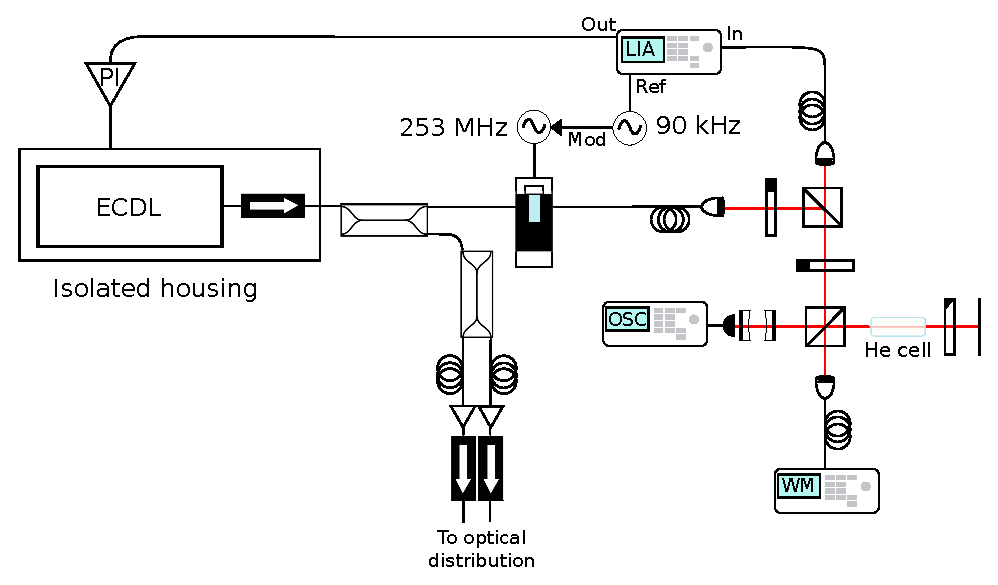
\includegraphics[width=\textwidth]{fig/apparatus/master_laser_system}
		\caption{Schematic of the generation and control system for the main cooling laser operating at 1083.331 nm described in the text. Light from the laser diode is filtered by the cavity resonance and internal diffraction grating, which is actuated by a piezoelectric crystal. Part of the light is picked off with an in-fibre beamsplitter and sent to the experiments. The rest passes through an in-fibre AOM which increases the frequency by 253 MHz and outputs light into the saturated-absorption spectroscopy system (lower right). The SAS offset is in turn modulated at 90kHz and the demodulated signal (output of the LIA) is proportional to the gradient of the SAS signal, which is minimized at the absorption peak. Hence the demodulated output serves as the error signal for a PID controller that feeds back to the piezoelectric actuator of the frequency-selective diffraction grating. Further details about the spectroscopy technique can be found in \cite{ShinThesis,FootAtomic}.}
		\label{fig:main_laser}
	\end{figure}
	
	
	The principal light source for both machines is the 1083.331 nm cooling and trapping laser.
	The light source, depicted in Figure \ref{fig:main_laser}, is an external-cavity diode laser (ECDL) that operates with a locked linewidth below 100 kHz and is detailed in the publication \cite{Shin16} and in PhD thesis of D. K. Shin \cite{ShinThesis}.
	The output of the ECDL passes through an in-fibre beamsplitter, from which one output is blue-shifted by 253 MHz by an acousto-optical modulator (AOM) and locked to a helium gas cell by saturation absorption spectroscopy.
	The remaining arm is coupled by optical fibres to the fibre amplifiers of both experiments.
	Each experiment features its own fibre amplifier that produces up to 5 Watts of laser power from the $\approx$3 mW supplied by the ECDL and then distributes the light to the laser cooling and trapping chambers via a suite of dedicated AOMs (depicted in section \ref{sec:new_optics}).

	
	% N Herschbach, Trrapped Triplet helium atoms: inelastic collisions and evaporative cooling, PhD thesis VU Amsterdam 2003


	% http://www.heliumbec.com/wiki/February_2017_Bake
	% https://imgur.com/a/4BxKh
	% http://www.heliumbec.com/wiki/Titanium_Sublimation
	% \begin{figure}
	% 	\centering
	% 	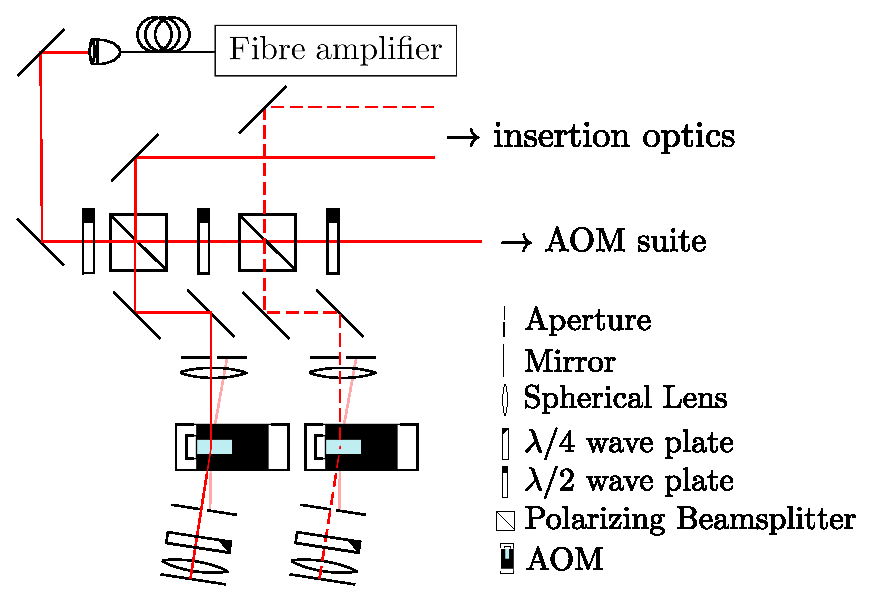
\includegraphics[width=0.6\textwidth]{fig/apparatus/distribution_optics}
	% 	\caption{Partial schematic of the control and distribution system for cooling light in the lattice machine. The fibre amplifier supplies light to each of several AOMs in cat's-eye configuration (two shown, one marked with dashed beamline). Half-wave plates control the optical power supplied to each AOM via polarizing beamsplitters. Pairs of mirrors permit alignment through a focus lens into the AOM crystal. The first diffracted mode is spatially selected by an aperture on the outgoing side, which is reflected and re-focused by a lens of equal focal length. A quarter-wave plate ensures that the the polarization is rotate from H to V after the second pass through the AOM hence is transmitted through the beamsplitter and then to the beam-forming optics before insertion into the vacuum chamber. }
	% 	\label{fig:distribution_optics}
	% \end{figure}

	In each machine, a suite of AOMs are used to independently control the power and frequency of each of several specialized beams\footnote{The active component of an AOM is a crystal is driven at radio frequencies by an amplified voltage-controlled oscillator.	An acoustic standing wave, constituted by phonons with frequency matched to the driving frequency, scatters light into discrete diffraction modes width momenta shifted by the phonon-lattice momentum.	The action is analogous to a diffraction grating, and described by the Kapitza-Dirac mechanism.	Thus the AOM transduces electronic signals into optical frequency shifts.	An analogous effect, with the role of atoms and light interchanged, is the operating principle of optical lattices.}.
	The AOM suites are supplied by light picked off from the output of the fibre amplifier by a half-waveplate and beamsplitter pair per AOM.
	The first-order diffraction is usually chosen for its more efficient transmission.
	The pointing of the diffracted beams vary with the AOM frequency, which is a problem when the ultimate destination of the light is separated from the AOM by several meters of optical path length, after which the deflection can become significant.
	To circumvent this, the AOMs are set up in a double-pass ``cat's-eye" configuration so the deflection in one pass is canceled by the second pass in the opposite direction.
	A quarter-wave plate placed in the optical path through the cat's-eye ensures the doubly-diffracted beams are transmitted back through the beamsplitter into the distribution optics.
	
	AOMs offer the advantage of fast switching times, but some light can leak from the AOM suite through the optical paths into the vacuum chamber.
	As such we used electronic shutters and an opaque enclosure to prevent this from occurring.
	The shutter action as well as the detuning and diffraction efficiency of the AOMs are actuated by the control software described later in this chapter.
	
	The supply of light which is 253 MHz red of the field-free resonance reduces the risk of stray light interacting with atoms and disrupting the delicate cooling and trapping processes.
	Furthermore, the fact that AOMs are limited in operation to a maximum frequency on the order of a hundred MHz or so means that the large detunings required for certain laser cooling applications could not be achieved using such double-pass setups seeded by resonant light\footnote{Cascading double-pass systems are certainly possible, but adding more moving parts with efficiencies generally below 80\% is undesirable.}.
	The lattice machine also makes use of 1550nm light for trapping in an optical dipole (and eventually lattice), whose generation and application is discussed in appendix \ref{chap:lattice}.	


	
	

\subsection*{Spectroscopic laser}
%mark
\label{sec:spec_laser}
	\begin{figure}
		\centering
		\includegraphics[width=\textwidth]{fig/apparatus/exp_optics_schematic}
		\caption{Schematic of the spectroscopic laser system.  The main laser modules supply light through an optical fibre, after three stages of optical filtering, to the insertion optics. The input to the fibre is the first diffraction mode from the AOM that serves as the actuator for an electronic PID loop whose power set point (P set) is compared to the reading of a photodiode (P act) at the insertion optics. The laser frequency is stabilized by a software-based PID loop that actuates the Ti:S cavity length (via inboard piezos) to reduce the between the desired and actual wavelengths ($\lambda$ set and $\lambda$ act, resp.). A pair of scanning Fabry-Perot cavities (SFP)  monitor the light from each laser module to verify both are operating in a single-mode regime. The switches at the input to the Ti:S are shown in the configuration used to calibrate the wavemeter. In this procedure the flipper mirror (coupling red light to the SFP) is removed and light enters a cesium gas cell. The fluorescence signal is measured by a photomultiplier tube backed by a photodiode, and this provides the signal for a dither lock at 1 kHz, demodulated by a lock-in amplifier (LIA).}
		\label{fig:tunable_laser}
	\end{figure}

	A light source unique to the BiQUIC machine was the tunable laser system used to generate light in the $402-430$ nm range for laser spectroscopy (namely the works \cite{Ross20,Henson22} corresponding to chapters \ref{chap:transitions} and \ref{chap:tuneout} respectively, and also Ref. \cite{Thomas20}).
	This laser system is depicted in Figure \ref{fig:tunable_laser}.
	Light at 1064nm from a Lighthouse Photonics \emph{Sprout} module was frequency doubled by second-harmonic generation to pump an M-squared SolsTi:S titanium-sapphire laser which we operated around 800 nm.
	The output from the SolsTi:S was doubled again in an M-squared ECD-X module to the target wavelengths.
	A fraction of the light is fed into a High Finesse WS-8 wavemeter.
	A MATLAB software lock uses the wavemeter output to stabilize the laser to within 100 kHz of the target wavelength, and allows automatic scans across the region of interest by automatically updating the laser set point (details are provided in section \ref{sec:DAQ}).
	We use the wavemeter to lock the tunable laser with respect to the red light, so the instrumental uncertainty is doubled in determinations of the blue frequency.
	High Finesse specifies the absolute accuracy of the WS-8 at 2 MHz within 2 nm of a transition line, and 10 MHz otherwise.
	We calibrated the wavemeter once every day or so with respect to the two-photon crossover transition between the $6^2P_{\frac{3}{2}} (F=4)$ and $6^2P_{\frac{3}{2}} (F=5)$ lines in a cesium vapor cell.
	We used saturated absorption spectroscopy to lock the red light to the Cs transition while feeding light into the wavemeter for the calibration.	
	

	We used the first diffracted mode of an AOM, driven at 189 MHz, to control the beam power.
	The output of the AOM was fed into an optical fibre which coupled the light to the vacuum insertion optics.
	{After exiting the fibre, the light was linearly polarized and a small fraction was directed onto a photodiode, whose voltage served as the input parameter to a PID loop.
	The control loop had a 3dB bandwidth of 170 kHz and was able to stabilize the beam power to within a relative error of 0.3\%.}
	There, we used waveplates to set the polarization and a telescope to magnify the beam up to $\approx$2 cm waist.
	A final lens fixed to a three-axis translation mount was used to focus and align the beam.
	For the measurements of the tune-out and forbidden transition wavelengths, we focused the beam to a $\approx10~\mu$m diffraction-limited waist at the site of the BEC to achieve strong interaction given the weak signals of interest.
	For the $2\triplet P_2\rightarrow 5\triplet D$ transitions described in chapter \ref{chap:transitions}, the beam was collimated and operated at a reduced power to mitigate power broadening and saturation of these much stronger resonances.
	The optical power was regulated with reference to a photodiode that sampled the beam after the fibre via a polarizing beamsplitter.

	The wavemeter logs, photodiode voltage, and transmission of light from both the red and blue beams through two scanning Fabry-Perot cavities (SFPs) were recorded through the DAQ system in order to provide diagnostics in post-processing.
	Part of the data analysis pipeline then automatically discarded shots where either SFP showed multiple peaks within a single free-spectral range (FSR), indicating that one of the lasers was running in a multimode regime, or where the photodiode trace indicated a laser supply failure, or where other anomalous behaviour was detected.

% \rem{\subsubsection{Wavemeter Calibration}
% 	To provide an absolute calibration of the wavemeter we use the Doppler-free two-photon $6^{2}S_{1/2} (F=3) \rightarrow 8^{2}S_{1/2} (F=3)$ and $6^{2}S_{1/2} (F=4) \rightarrow 8^{2}S_{1/2} (F=4)$ transitions in cesium around 364.5~THz (822.5~nm). We split off a small fraction ($\sim$50~mW) of the red light generated by the Ti:Sapphire laser (before the doubling cavity), pass it through a warm (50$^{\circ}$~C) cesium cell with a beam waist of $\sim0.5$~mm, and then reflect it backwards along its path.
% 	We detect the excitation of the transition using the blue florescence from the radiative cascade \cite{Hagel99}, with a blue-sensitive (red-blind) photomultiplier tube (PMT). Previous measurements \cite{Wu13,Fendel07} have precisely measured the $F=3\rightarrow3$ and $4\rightarrow4$ transitions to be 364\,507\,238.363(10) and 364\,503\,080.297(10) MHZ respectively, and have demonstrated an insensitivity to environmental conditions, which makes these transitions suitable as a secondary frequency standard. 

% 	To calibrate the wavemeter we disable the usual software based wavemeter feedback to the laser and instead stabilize the laser using one of these transitions. To produce a derivative error signal suitable for feedback we modulate the frequency of the Ti:Sapphire laser (frequency deviation $<50$~kHz, modulation frequency $\sim1$~kHz) and detect the resulting modulation in the PMT current with a lock-in amplifier. This analog error signal is continuously read by a software based PID controller which sends adjustment commands to the laser controller (rate $\sim20$~Hz) to maintain the the laser frequency at the maximum of the fluorescence.

% 	As a verification of the calibration procedure we then re-engage the wavemeter based laser feedback system and measure the PMT current as a function of the frequency set point. We fit these data with a Lorentzian profile to extract the transition frequency and verify the calibration procedure (see Fig.~\ref{fig:2p_scan_single}). After calibration we find that measurements of both $F=3\rightarrow3$ and $F=4\rightarrow4$ transitions give frequencies within 50~kHz of the reference values.
% 	Calibrations are carried out every few days as the ($\sim100$~mK) temperature stability of our laboratory reduces the thermal drift of the wavemeter.
% 	Based on previous systematic studies of these transitions \cite{Wu13,Fendel07} and the conditions used for calibration, we believe that the systematic error of this calibration procedure ($<100$~kHz) is well below the absolute accuracy of the wavemeter over the measurement range used in the this work (2~MHz within 3~THz (2~nm) of calibration \cite{wstechnical}). As the wavemeter measurement and calibration is carried out on the red side of the laser system before the doubling cavity the absolute accuracy of the frequency of the delivered (blue) light is doubled to 4~MHz, well below other systematic uncertainties.

	% references for 2p transtion
	% https://www.osapublishing.org/ol/abstract.cfm?uri=ol-32-6-701
	% https://www.osapublishing.org/ol/abstract.cfm?uri=ol-30-24-3413
	% https://www.sciencedirect.com/science/article/pii/S0030401898006622?via%3Dihub#FIG3
	% https://www.osapublishing.org/ol/abstract.cfm?uri=ol-38-16-3186


	% \begin{figure}
	%     \centering
	%     \includegraphics[width=0.6\textwidth]{fig/tuneout/2p_scan_nice}
	%     \caption{(Top) single scan of PMT current vs. optical frequency relative to the two photon transition $6^{2}S_{1/2} (F=3) \rightarrow 8^{2}S_{1/2} (F=3)$. A Voigt fit is shown as the black line for comparison, with fit parameters are $\sigma=0.18(3)$~MHz $\gamma=0.49(3)$~MHz. This scan took a total of \(75\)~s. (Bottom) Residuals of the fit model, where the shaded region is the standard deviation of the observation error model. 
	%     }
	%     \label{fig:2p_scan_single}
	% \end{figure}}
	% Camera/mirror setup Reproducibility
	% issues

\section{Detection of metastable helium atoms}
\label{sec:he_detection}
	Two optical detection methods are employed in the ANU helium labs.
	Resonant absorption imaging is only used in the lattice machine, and is therefore discussed in appendix \ref{chap:lattice}.
	Both machines make use of saturated fluorescence measurements to measure the number of atoms in a trap.
	In this method, bright resonant light ($I\gg I_\textrm{sat}$) is applied to the atoms such that the population of the excited state saturates at 50\%.
	If the light is applied while the trap remains on, then while some atoms may decay to a trapped state, repeated absorption events eventually drive them out of the trap.
	Therefore, one expects a sharp peak and subsequent decay in the optical power re-emitted from the trap.
	This radiation can be captured by a lens and focused onto a photodiode, producing an analog voltage which can be used to measure the number of atoms confined in the trap.
	The difference between peak and steady-state voltage after the pulse is a direct probe of the atomic population (see appendix \ref{chap:lattice} for further discussion).
	This technique is employed as a diagnostic tool for fast readout of the second MOT population when optimizing the alignment of cooling and trapping beams. 

	A unique diagnostic available in helium experiments is the production of helium ion-electron pairs.
	This process can be monitored by in-vacuum electron multipliers mounted near the trapping region.
	Proximity to the trap is desirable for efficient collection of the resulting particles.
	Aside from investigating Penning ionization itself, ion detection has been applied in photoassociation spectroscopy \cite{Herschbach00,Koelemeij04}, to monitor the onset of Bose-Einstein condensation \cite{Tychkov06}, and for high-precision laser spectroscopy \cite{Rengelink18}.
	Ion detection garners only a brief mention in works relevant to appendix \ref{chap:lattice}, wherein we hoped to detect ions as a diagnostic when aligning an optical dipole trap\footnote{The ion detector in the BiQUIC machine stopped working some years ago and has not been replaced: the utility of this diagnostic is outweighed by the effort required to break vacuum for the first time in a decade or so, disassemble the chamber and surrounding optics, reassemble everything, bake the chamber, and realign all the optics.}.
	In an accident a year or so after I left that lab, a ceramic feed-through connecting the ion detector to the external electronics cracked.
	This broke vacuum, necessitating a rebake of the chamber, and saw the detector retired.
	


\subsection*{Single-atom detection with the MCP-DLD stack}
	\label{sec:DLD}
	% http://www.heliumbec.com/wiki/Detectors
	The principal detection scheme in this thesis is single-atom sensing in the far-field regime using a multichannel plate and delay-line detector combination (MCP-DLD)\footnote{In this context far-field means that the density of the cloud is determined by the initial velocity distribution and that effects of the finite initial size are negligible. This is suitable in our experiments because the condensate is smaller than the detector resolution. See chapter 5 of D. K. Shin's PhD thesis \cite{ShinThesis} for a quantitative discussion.}.
	

	\begin{figure}
		\centering
		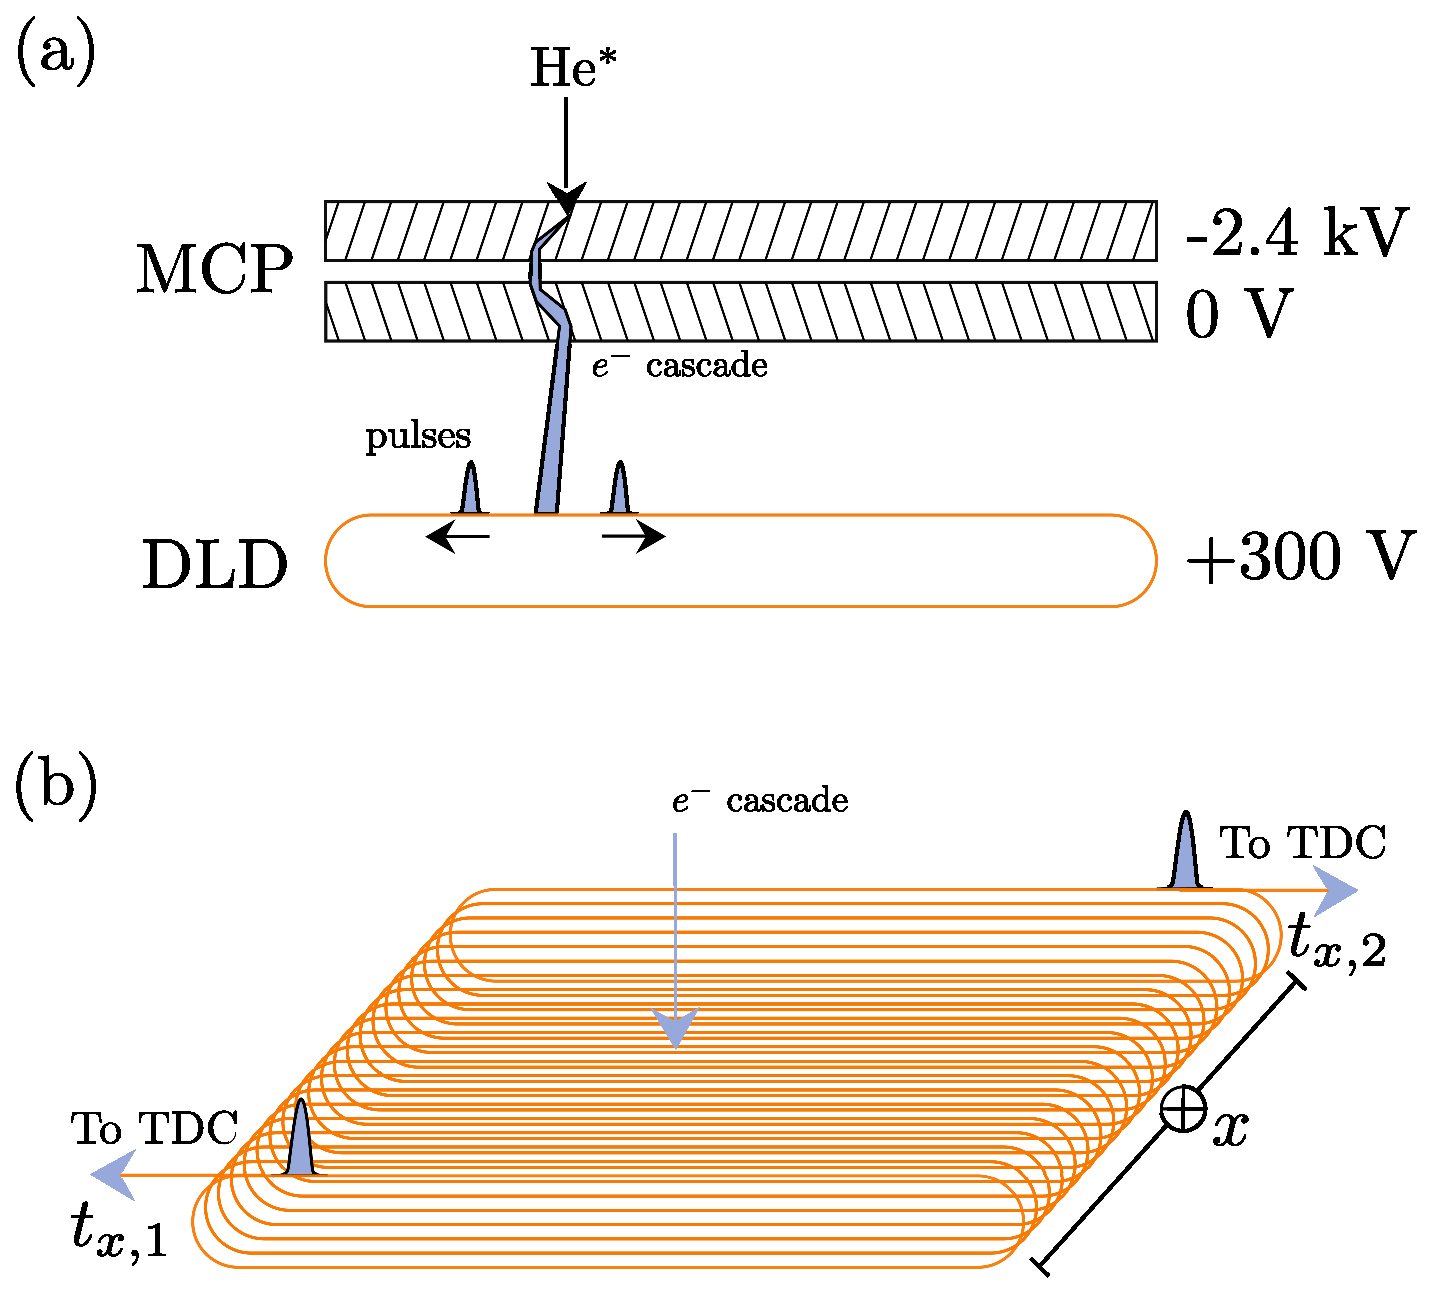
\includegraphics[width=\textwidth]{fig/apparatus/mcp_dld_schematic}
		\caption{Schematic sketch of the MCP-DLD detector. The twin plates of the multi-channel electron multiplier (MCP) have a 2.4 kV potential between the upper and lower surfaces which accelerates electrons along the pores after they are freed from the surface by the energy released from \mhe~impact events. The resultant shower of electrons deposits a charge excess on a winding of the delay-line detector (DLD), which disperses as oppositely-travelling current pulses along the line. The arrival times ($t_{i,1}$ and $t_{i,2}$) of each pulse along each axis are received by the TDC and used to infer the respective coordinate of the electron cascade (only the winding along $x$ is shown for simplicity, but in the BiQUIC machine the DLD consists of two orthogonal windings).}
		\label{fig:MCP_DLD}
	\end{figure}

	In some configurations, such as the one at the \mhe~group at VU Amsterdam, the MCP itself can be used as an ion- or metastable-atom detector.
	In our machines, the MCP is paired with either a phosphor screen (usually only used for diagnostic purposes) or more typically with a delay line detector to form the MCP-DLD that is the workhorse of most experiments conducted at ANU.
	A summary description is given here, and detailed explanations of the detector stack and signal processing pipeline can be found in \cite{ShinThesis, HodgmanThesis, ManningThesis}.
	The MCP consists of two plates, each of which feature 10 $\micron$-diameter pores arranged in a square grid with 20 $\micron$ between the centres of the pore openings.
	The plates are 80 mm in diameter, with the upper surface 848 mm below the BiQUIC trap centre.
	The freefall time-of-flight of the centre of mass of the cloud is 417 ms, and so the maximum detectable horizontal velocity is about 9.5 m/s, sufficient to capture almost all of the thermal fraction for clouds below the critical temperature.
	The detector plates are grounded for most of the experimental sequence, and then the top plate is ramped to $-2.4$ kV over about 2 seconds before dropping the trap.
	The negative voltage repels electrons from the surface of the plate, protecting the detector surface from degradation and reduces the background count rate.
	The background rate, also called the \emph{dark count} rate, is typically 0.56 Hz/cm$^2$ when operating the plates at $-2.4$ kV, and is negligible for the purposes of experiments in this thesis.
	

	When an atom strikes the surface of a pore after falling from the trap, a second-order process releases a free electron with most of the 19.8 eV as kinetic energy \cite{Jagutzi02,Hotop96}.
	These electrons are accelerated down the pore by the strong electric field, and themselves impact the pore surface and eject more electrons, triggering an electron avalanche that amplifies each atom impact into over 10$^6$ electrons.
	The electron shower exits the back of the detector and is accelerated by a +300 V potential towards the delay-line detector (DLD).
	The DLD in the BiQUIC machine consists of two coils of wire each wound in a helical pattern and arranged perpendicular to one another.
	 The arrival of an electron cascade causes a current pulse to travel along each wire in both directions from the point of impact.
	The pulses pass through a fast pre-amplifier and then through a constant-fraction discriminator which converts the analog pulses into a digital signal.
	Both of these processes take place within a Roentdek DLATR6 which is located outside the vacuum chamber.
	The digital pulses are transmitted to a Roentdek TDC8HP time-digital converter (TDC) which registers the arrival times, relative to the arrival of the main trigger signal from the LabView control software, and writes these to a \verb|txt| file as \verb|(channel,time)| pairs.
	Finally, a custom C++ script passes over the file and converts the timing data to \verb|(t,x,y)| tuples.
	The conversion from \verb|(channel,time)| to \verb|(t,x,y)| is performed separately, and indeed the latter usually by a different machine, so as to provide maximum CPU availability to the acquisition function.	Further details about the architecture, construction, and calibration of these detectors is found in \cite{HodgmanThesis,ManningThesis}.

	A second MCP, backed by a phosphor screen and a mirror at 45$^\circ$ to the vertical axis, is mounted on an in-vacuum translation stage below the main chamber.
	The mirror directs light from the phosphor screen to a CCD camera mounted outside the vacuum chamber.
	This detection method is not typically used for scientific purposes these days, but is a useful additional diagnostic when the MCP-DLD detector stack appears to be faulty.
	The phosphor screen does have a much larger dynamic range than the DLD, however, which makes it useful for visual spotting of subtle distortions in the BEC profile, such as used in the alignment of the spectroscopic probe beam.
	


	% % NTM [185] derivation of detector flux profiles - inc mean field 
	% % % Tychkov PhD thesis
	% % RGL [98] calibration of QE - depends on plate voltage, which in turn affects plate lifetime and rate of degradation of QE 
	% % % van Rooij PhD thesis
	% % RGL MCP flux models [94] inc BEC flux in terms of chemical potential 
	% % % van Rooij PhD thesis
	% % TKV [9,10] expanding condensate density distributions 
	% % % Y Castin, R Dum, bose-einstein condensation in time-dependent traps, Physical Review Letters 77, 1996
	% % % F Dalfovo, S Georgini, L P Pitaevskii, S stringari, theory of bose-einstein condensation in trapped gases, rev mod phys 71, april 1999
	% % SSH [38,39] condensate ballstic expansion 
	% % % Castin & Dum
	% % % K.
	% Dieckmann, Bose-Einstein Condensation with High Atom Number in a Deep Magnetic Trap, Ph.D.
	% thesis, University of Amsterdam (2001).

		 % \newpage
	 \begin{figure}
	 	\centering
	 	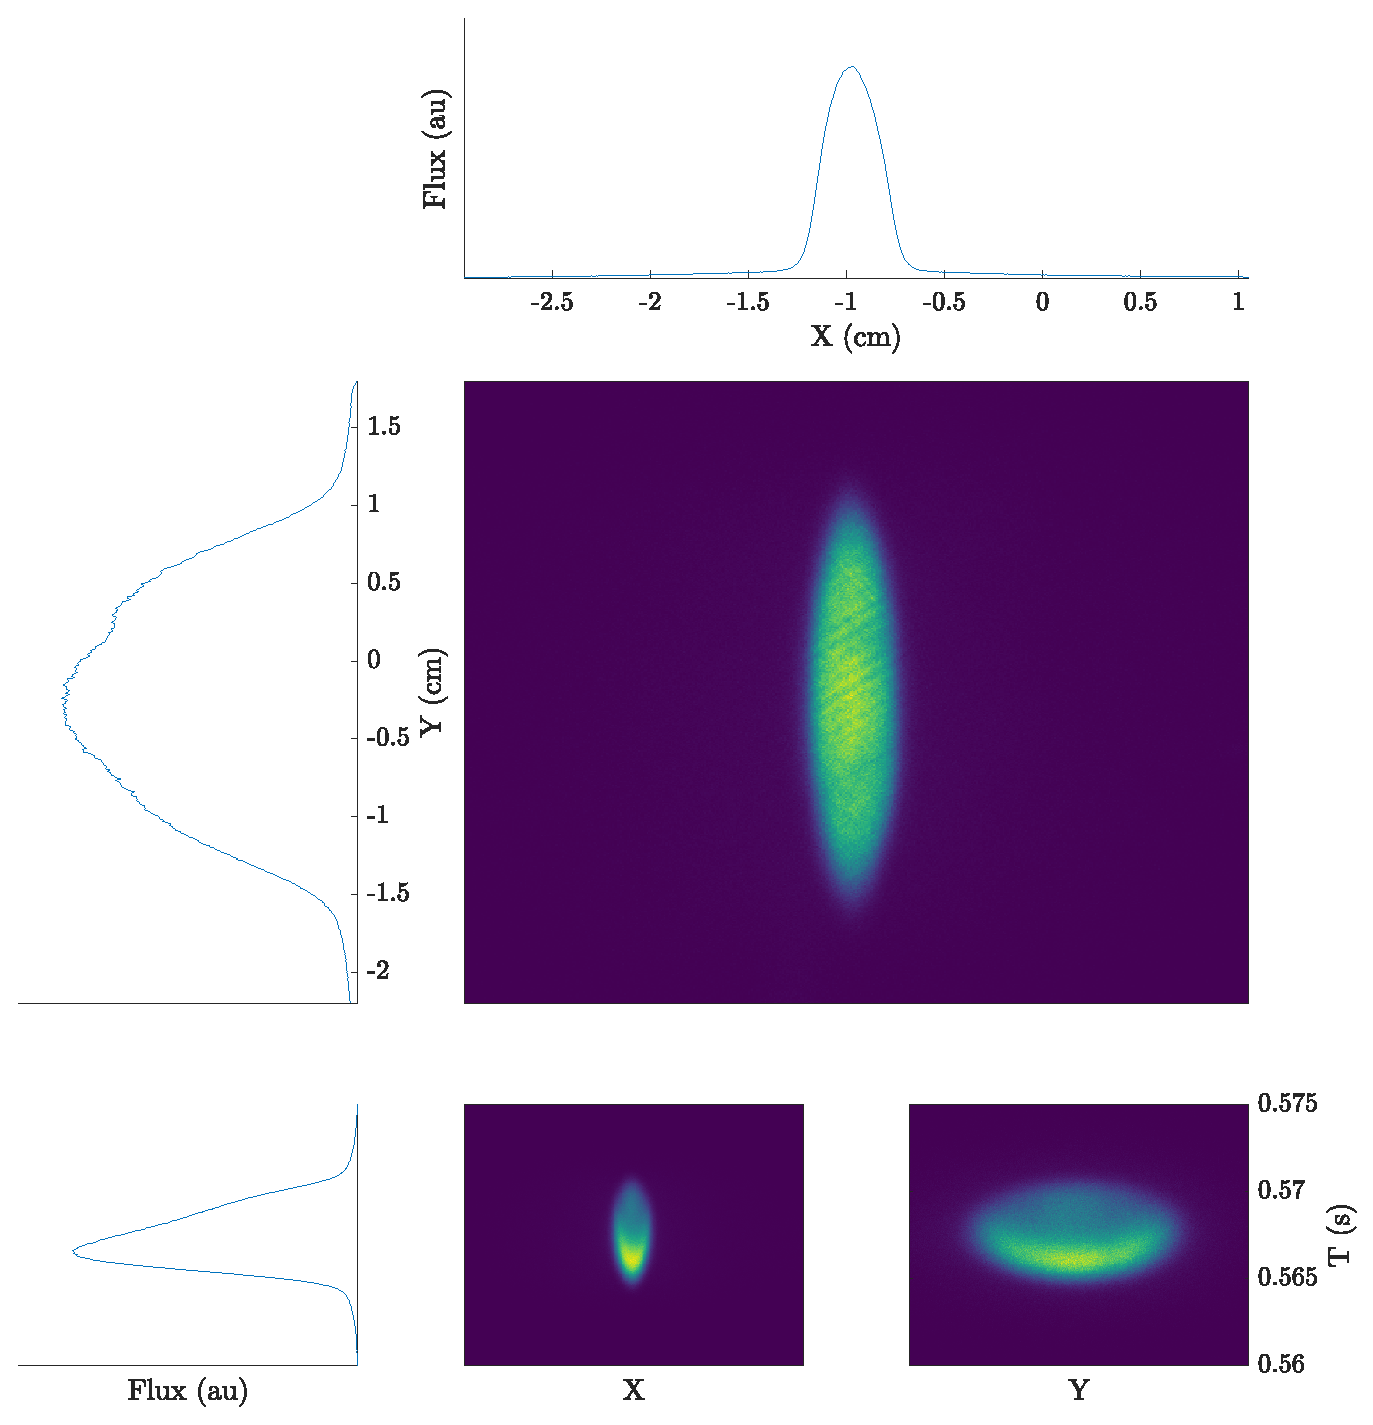
\includegraphics[width=\textwidth]{fig/apparatus/dropped_bec}
	 	\caption{MCP readout of a dropped BEC with small thermal fraction, just visible as dilute wings outside the central peak.
		The detector saturation is evident in the time-of-flight profiles (bottom row, all with common vertical axis) as a sudden downturn in the detected flux, whereas the full BEC has a parabolic profile.
		The density- and space-dependence of the saturation is visible in the 2D sections (lower middle and lower right). The one-dimensional fluxes along X and Y are averaged over the time interval displayed in the bottom row, and the total count rate (bottom left) is integrated over the entire detector.}
	 	\label{fig:dropped_bec}
	 \end{figure}

	 \newpage
	 \begin{figure}
	 	\centering
	 	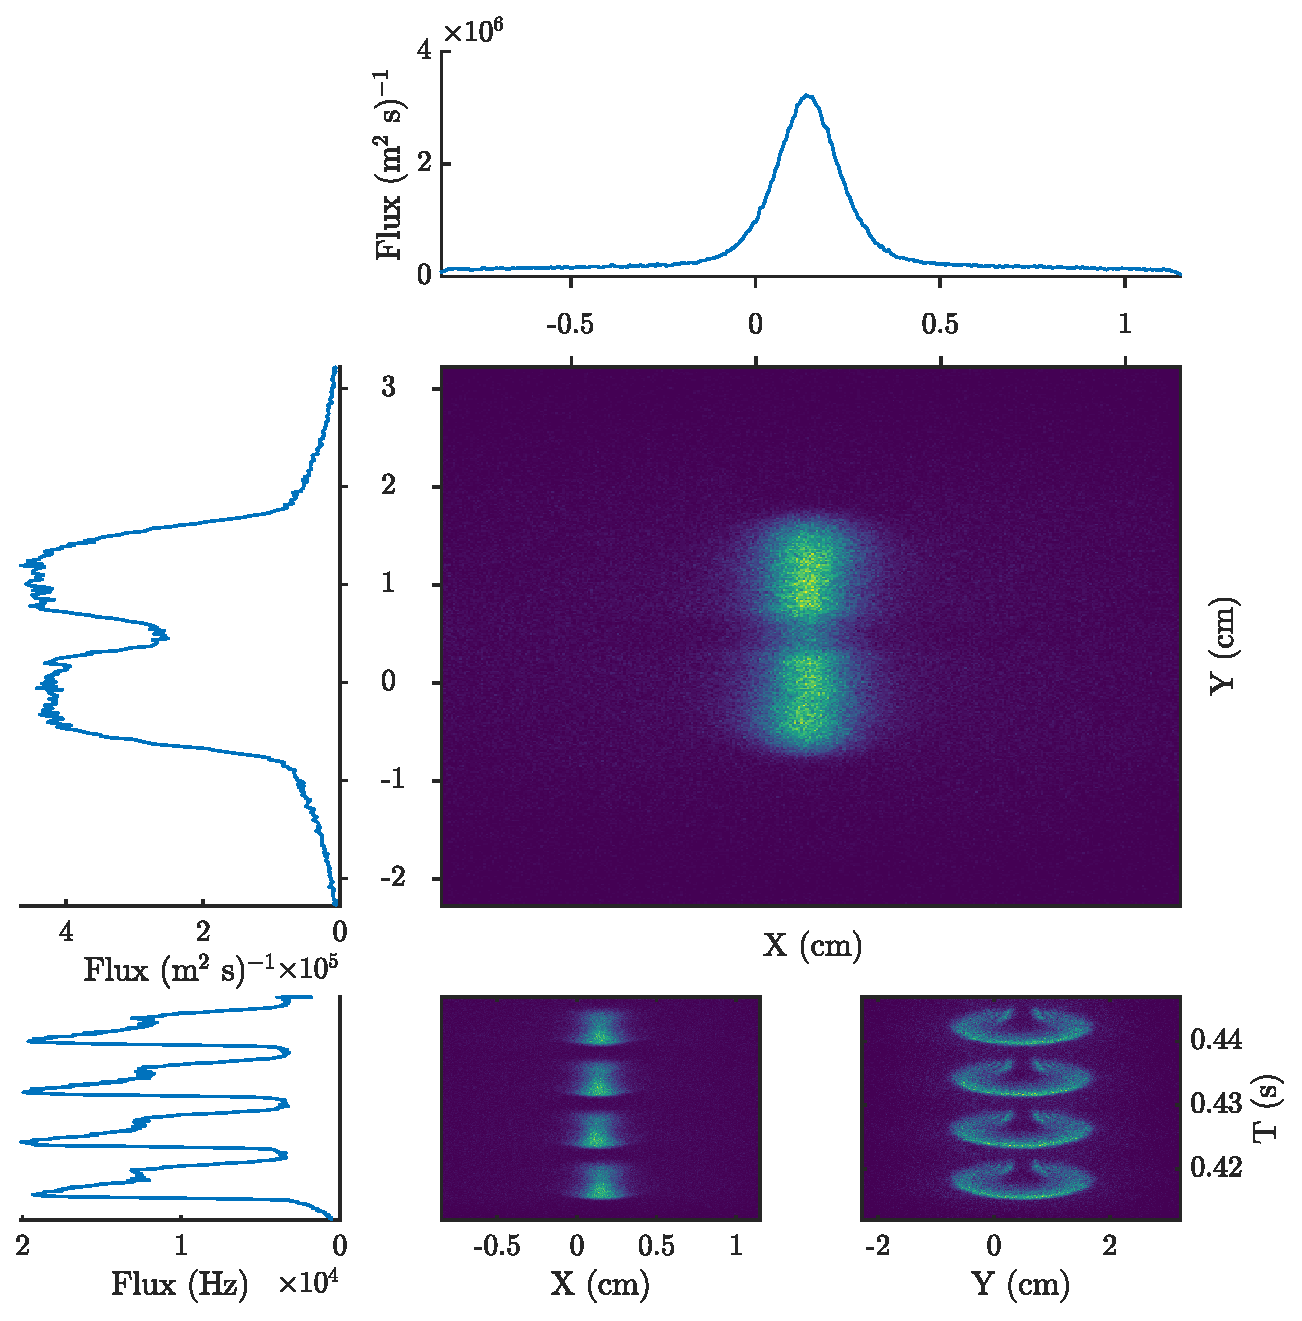
\includegraphics[width=\textwidth]{fig/apparatus/dropped_pal}
	 	\caption{MCP readout of the first few pulses from a pulsed atom laser, displayed similarly to Fig. \ref{fig:dropped_bec}. When atoms are transferred into the untrapped state, they are repelled from the trap by the mean-field energy of the remaining condensate, leading to pulse broadening especially in the tight $(y,z)$ axes. In the dilute outcoupled pulse, the speed of sound is low enough that the relative velocity of the pulse and BEC is supersonic in the outcoupled cloud, leading to the complex interference patterns which have been identified as \emph{Bogoliubov-Cerenkov radiation}\cite{Henson18_BCR}. The peak flux is about a thousandth of that for a dropped BEC, and hence saturation is avoided.
	 	% \footnote{This can be verified in two ways: One, for BECs of $N_0$ atoms, and variable outcoupling rate $\beta$ the pulse populations $N_i$ are proportional to the outcoupling rate. Two, within a single shot and fixed outcoupling rate $\beta$ the pulse populations decay geometrically, which would not be true were saturation evident in the earlier pulses.}. 
	 	The flat top of the Y-projection is due to the distortion of the profile during the trap escape, not detector saturation.}
	 	\label{fig:dropped_pal}
	 \end{figure}
	 \newpage

\subsection*{Atom lasers}
	\label{sec:atomlaser}


	% 	NB - the Einstein coefficients have a cubic dependence on frequency (See also the natural lifetime) and so optical transitions tend to exhibit spontaneous decay more quickly than the Rabi oscillations, but radio transitions (as in the fine structure states) fall much more slowly and coherent oscillations can be seen 
	% One can see that at large detunings, the oscillation frequency ncreases but the amplitude falls off like the detuning-squared, and one instead encounters the dipole potential, right?

	The most straightforward way to use an MCP-DLD to interrogate a BEC is simply to drop the atoms onto the detector.
	An example of this straightforward detection scheme is illustrated in Fig.
	\ref{fig:dropped_bec}.
	A drawback of this method is that the high atom fluxes in large BECs can temporarily deplete the available current carriers near the surface of the detector, resulting in a nonlinear reduction in detection efficiency known as \emph{saturation}.
	This means that for even moderately sized condensates, a determination of the condensate population by counting detection events or by straightforward fitting of the time-of-flight profile is impractical, and one cannot compute interesting quantities like correlation functions with meaningful accuracy.
	Another limitation of the trap-release method is that it is a completely destructive measurement - one cannot re-trap the cloud or only drop part of it, which slows down data acquisition for even simple purposes like determining the trapping frequencies.
	Atom lasers can circumvent both of these issues.
	

	The basic principle of an atom laser is to transfer some portion of the condensed atoms into a state that is no longer confined by the trapping potential.
	This was first achieved (shortly after the first realisation of BEC) by applying pulses of RF radiation to a magnetically trapped condensate \cite{Mewes97}.
	Later, a continuous-wave atom laser was demonstrated and used to perform RF spectroscopy of the cloud, revealing the symmetry-breaking action of gravity which pulls the BEC away from the minimum of the magnetic field \cite{Bloch99}.
	Optical Raman transitions\footnote{In atom optics, \emph{Bragg} transitions, which impart a momentum transfer, are distinguished from  \emph{Raman} transitions which induce a change in the electronic state.} can also be used as the outcoupling mechanism \cite{Hagley99} with the advantage of imparting a controllable momentum to the outcoupled atoms, but are not employed in the works in this thesis.
	

	Atom lasers are so named because the trapped condensate acts as a reservoir of coherent matter waves, in analogy to lasers as a source of coherent light \cite{Naraschewski99,Glauber63}.
	The first-order coherence of atom lasers is evident from the observation of interference fringes between matter-wave beams \cite{Andrews97} and the higher-order coherence manifests in the many-particle correlations detected in \mhe~atom lasers \cite{Manning10,Dall11a,Rugway11}.
	Atom lasers can also be collimated \cite{Bloch99}, directed with collimated laser beams playing the analogous role of an optical waveguide \cite{Guerin06,Couvert08}, and manipulated with optically-induced `mirrors' and beamsplitters \cite{Bloch01}.
	The potentially continuous operation of atom lasers \cite{Chikkatur02} brings the analogy with conventional lasers even closer.
	Atom laser physics has been studied in detail and widely deployed through the field of atom optics in the two intervening decades since their conception, including all of the experiments described in this thesis.
	
	% NB this Andrews paper makes some interesting points about the nature of the condensate order parameter, arrguments about whether BEC is actually coherent/hhas a phase, and the relationship between gauge symmetry breaking and particle number conservation - c.f.
	% that recent paper about number fluctuations in a condensate, discuss in overview


	A simple explanation of the mechanism of an atom laser requires a two-level atom with magnetically trapped and untrapped states labeled $\ket{1}$ and $\ket{0}$.
	An RF pulse tuned to the splitting $\omega_{10}$ induces an oscillation between the two states with Rabi frequency $\Omega$ for a duration $t$.
	For an ensemble of $N$ atoms, the independent single-particle oscillations produce a many-body product state which evolves as \cite{Mewes97}
	\begin{align}
		\ket{\Psi} &= (\cos(\Omega t/2)\ket{0} + \sin(\Omega t/2)\ket{1})^{\otimes N} \\
		& = \sum_{n=0}^{ N}\sqrt{\frac{N!}{n!(N-n)!}}\cos(\Omega t/2)^{N-n}\sin(\Omega t/2)^n\ket{N-n,n},
		\label{eqn:PAL_Rabi}
	\end{align}
	where $\ket{N-n,n}$ denotes the state with $n$ atoms coupled out of the trapped state and $N-n$ atoms remaining.
	The outcoupled fraction is then $\sin^2(\Omega t/2)$.
	% \footnote{There is the question of when the atoms actually leave the trap.
	% In one picture, the RF pulse simply allows the atomic wavefunction to couple periodically to the decay channel corresponding to collision with the detector.
	% So they don't actually 'leave' the trap until there's a detection event.}.

	In practise, the Zeeman splitting varies across the trap due to the inhomogeneous magnetic field, and so a narrow RF pulse would only be resonant with a section of the condensate.
	While useful for detailed spectroscopy of the condensate, the outcoupling rate would depend on the condensate population.
	This can be circumvented by applying short RF pulses resonant with the minimum Zeeman splitting of the trap.
	If such pulses are sufficiently short, the Fourier broadening of the finite-duration pulse is wider than the RF width of the condensate.
	The typical radio-frequency width of the condensate, i.e.
	the difference between the resonant frequency at the centre and the edge of the condensate, is set by the chemical potential of the condensate and is typically less than 10 kHz in our experiments.
	The outcoupling pulse typically consists of 6-10 cycles of RF tuned to the Zeman splitting of the trap bias, which typically ranges from 0.6-1 MHz depending on the configuration that is most suited to the experiment at hand. 
	This leads to pulses that range from about 5-25 $\mu$s, where the number of cycles is the most direct means to control the outcoupling rate (c.f. Eqn. \ref{eqn:PAL_Rabi}).
	An example of the MCP-DLD readout from a pulsed atom laser is shown in Figure \ref{fig:dropped_pal}.

	% Therefore, an RF pulse duration of order X sec is sufficient to ensure a uniform transfer across the trap.
	
	
	 % The pulses typically on the order of 100$\mu$s long, which for a typical trap splitting of order 2MHz ensures the spectrum of the pulse has a FWHM of order xMHz thanks to Fourier broadenin.
	


% PAL picture is integrated over 156 shots from 5_3d_2_3 data
% QD picture is integrated over about 1300? in tight trap fwiw from run 8

% PAL parameters; 1.6-3 MHz centering (see that ol plot) depending on trap
% pulsees 6-12 cycles
% typically sampled at 6-11 ms periods, generally limited by BEC width
% 




	


\section{Data acquisition \& control}
\label{sec:DAQ}
	
	Control of the optical components, coil current supplies, and RF radiation is coordinated by a central LabView program which transmits pulse sequences to the machine via National Instruments pulse generation cards.
	The cards themselves are connected to the CPU by a PCI bus, and synchronize their internal clocks at the beginning of each shot.
	The cards also record analog inputs such as Fabry-Perot cavity scan traces, photodiode traces, and mains voltage traces for post-processing diagnostics.
	The spectroscopic laser lock and tuning operations are also performed on the main control computer, as described in section \ref{sec:spec_laser}.

	The LabView control is supplemented by a command that calls a MATLAB subroutine (referred to as the `interface'), which is customizable to suit the purposes of a given experiment\footnote{The software developed to analyse the data from various experiments is invariably written in MATLAB.	Many core capabilities are stored in the repository \url{https://github.com/HeBECANU/Core_BEC_Analysis}, and generally each project will have a unique public repository as well.}.
	The motivation for this extension was for automatic and more flexible variation of experimental sequences. 
	This subroutine can return the \verb|.xml| file path of a LabView pulse sequence file for use in the next experimental cycle, and even modify the sequences, albeit in a limited way due to the particulars of LabView's sequence specification format.
	This extension allows for automatic optimization of experimental sequences, as was demonstrated in \cite{Henson18_ML}, but obviously is of no use for mechanical tasks like beam alignment\footnote{One can dream, though.}.
	Moreover, running back-to-back measurement and calibration shots would otherwise have to be done manually, as would updates of the spectroscopic laser wavelength during scans across the spectral region of interest.
	Therefore without the automatic update procedures enabled by the interface, the multi-day data collection runs embarked upon in this thesis would have become considerably more time-consuming and error-prone. 
	
	The interface script also writes metadata to a log file, including the POSIX timestamp, type of shot executed (e.g.
	\verb|calibration| or \verb|AtomLaser|), shot number, and other relevant parameters.
	The timestamps in this logfile can be cross-referenced with the \verb|txt| files that are written by the TDC computer and with the LabView logs of analog inputs in order to match the experimental parameters with data files for post-processing purposes.
	The data analysis pipelines for modern experiments can be complex, and the experiments in this thesis generally comprise a handful of different diagnostics processed in parallel.
	The tagging of shots by timestamp cross-referencing allows separation of relevant shots for each processing subroutine.
	
\subsection{Laser lock control protocol}

	As mentioned, the interface plays an important role in scanning the spectroscopic laser set point across regions of interest (be they electronic transitions as in chapter \ref{chap:transitions} or the tune-out wavelength in chapter \ref{chap:tuneout}). 
	The relationships between the subroutines involved in the laser control system are illustrated in Fig. \ref{fig:tcp_control}.
	The major features of this system architecture are two parallel processes which communicate with each other via MATLAB's cross-thread communication (\verb|labSend(data,to_process_id)| and \verb|labReceive(from_process_id)|).
	The messenger thread (T1) continuously looks for a TCPIP connection with the interface, which runs at the start of each experimental sequence and opens a TCPIP channel for the thread to connect with and receive the new setpoint.
	The control thread (T2) operates a PID loop by querying the wavemeter for its present reading (via USB connection) and also querying the laser control module for relevant parameters (particularly internal photodiode readings and voltages across piezoelectric actuators for interal optomechanics).
	The control loop then compares the desired set point to the measured set point and updates the actuator voltages according to the output of a discrete PID function.
	The control thread (T2) also contains a subroutine which is triggered when T1 sends the new setpoint through via \verb|labSend()| (which sets the \verb|labSend| bit to 1).
	If this condition is met, then T2 updates the setpoint for the PID loop with the new value obtained from \verb|interface| via T1.
	There is a stall condition here where the TCPIP port is opened by \verb|interface| but T1 is still waiting for the timeout of the last query, hence \verb|interface| will hang until the next loop of T1.
	This is not a major problem as the interface script must terminate before the pulse generation cards are triggered (they are sequential in the LabView program), so rather than interrupting the experimental execution it simply reduces the PID bandwidth briefly at the start of each run.
	The loop bandwidth is speed-limited by the frequent condition checks, device queries, MATLAB's limited speed as an interpreted language, and competition with other processes for CPU time. 
	Nonetheless the lock loop maintains a clock speed on the order of 10-15 Hz.
	The system has sufficient bandwidth to achieve a $\sim900$~ms rise time (10\% to 90\%) for a $\sim300$~MHz frequency step, and during interrogation we measured a typical (in-loop) standard deviation of 170~kHz. 
	The stabilization of the laser frequency uses measurements of the red side of the laser system (before the doubling cavity), so interruptions to the doubling cavity do not impact the lock.
	

	\begin{figure}
		\centering
		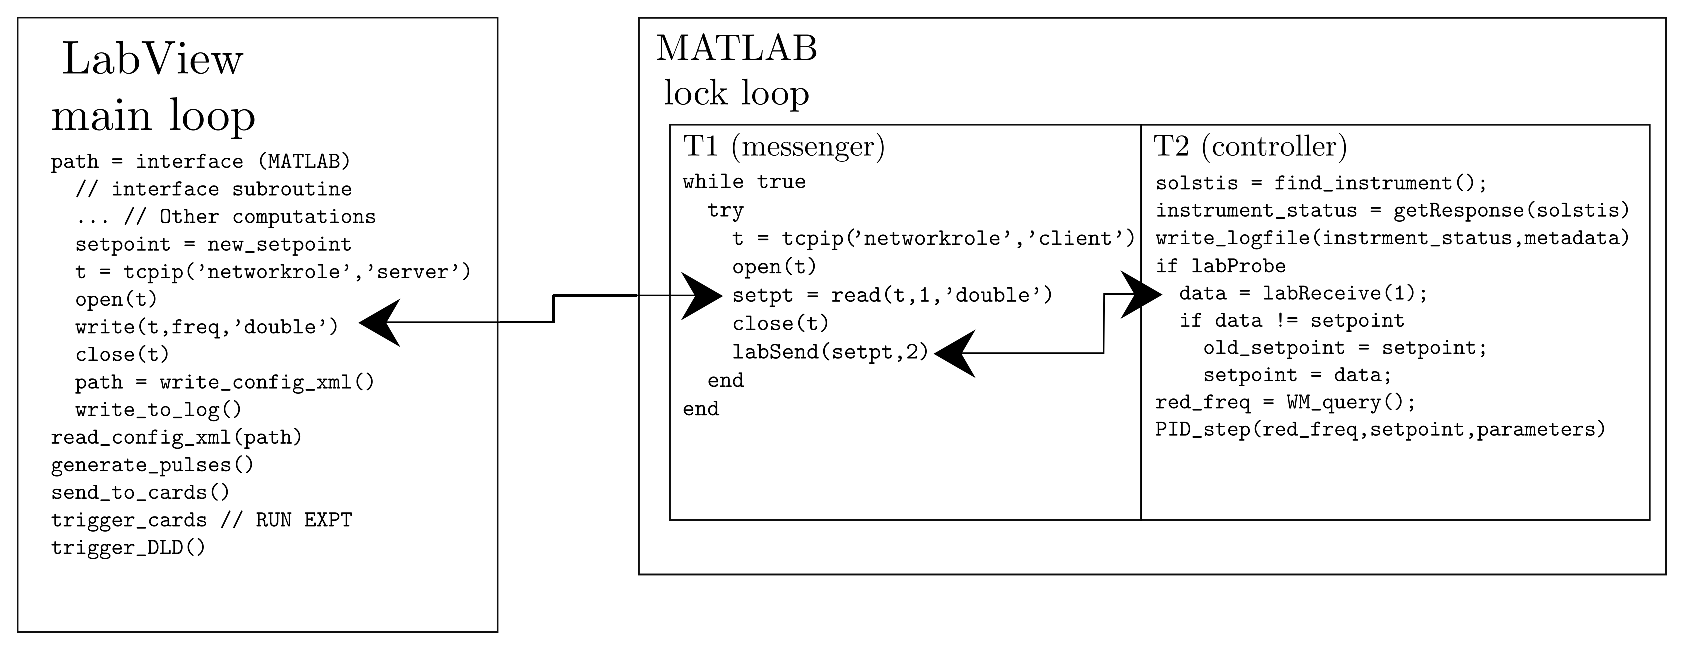
\includegraphics[width=\textwidth]{fig/apparatus/lock_loop}
		\caption{Schematic of the three major components of the lock loop used to scan the laser setpoint during spectroscopic measurements. As detailed in the main text, the main LabView script calls MATLAB subroutine which, among other tasks, communicates with a parallel pair of worker threads T1 and T2 which actuate the SolsTi:S controls.}
		\label{fig:tcp_control}
	\end{figure}




% tcpip interface for laser lock
% 	t = tcpip(IP, 33333, 'networkrole','server')
% 	fopen(t)
% 	fwrite(t,freq,'double')
% 	fclose(t)

% And on the other end - a loop that hammers it with queries?
% init parallel pool
% 	if workerID == 1
% 		while true
% 			try
% 				t = tcpip('localhost',33333,'networkrole','client')
% 				fopen(t)
% 				setpt = fread(t,1,'double')
% 				fclose(t)
% 				labSend(setpt,2)
% 			end
% 		end
% 	elseif workerID ==2 
% 		solstis = find_instrument();
% 		instrument_status = getResponse(solstis)

% 		write_logfile(instrment_status,metadata)
% 		% Omitting parameters for lock loop like wait times, slew rate limits, etc, various timers,

% 		if labProbe
% 			data = labReceive(1);
% 			if data != setpoint
% 				old_setpoint = setpoint;
% 				setpoint = data;
% 		red_freq = WM_query();
% 		PID_step(red_freq,setpoint,parameters)


% -> Something about communication between parallel workers?
% Ethernet link between PC and solstis driver; query returns machine state like internal photodiode readings and optomechanical actuator voltages


\subsection*{Optimizing machine performance}

	% Routine maintenance is required to keep the machine capable of producing large condensates.
	Despite the stabilized environment, optics are prone to wander slightly over time.
	The stable temperature is especially important as the cooling beams are coupled from the AOM tables to the vacuum chamber optics by free-space links.
	Drift in the relative position of the optics tables would therefore result in misalignment of many laser beams, and degrade performance of the machine.
	The conditioned air is supplied through three HEPA filters in the lab ceiling.
	The resulting positive pressure in an area enclosed by PVC strip walls keeps dust from entering the area on air currents.
	

	If the second MOT is loading and a saturated fluorescence signal is visible, one can usually optimize all of the optical alignments on this signal, which is a factor of ten faster than the full BEC creation sequence.
	If this is not available, logs of diagnostics taken at several points throughout the beamline can facilitate diagnosis of the point of failure.
	The most commonly employed tests are Faraday cups which produce a current when impacted by \mhe~atoms, as read out on a picoammeter.
	These current sensors are placed after the deflection stage, at the end of the Zeeman slower (with a large hole bored through it to allow the slowing beam to pass through), between the first MOT and the focus stage, and behind the second MOT chamber.
	In case the first MOT is not operational, a Xenics Bobcat CCD camera mounted above the chamber provides a view of the trapping region and direct visual feedback about the presence, shape, and density of the MOT.
	


	% A more elegant solution could take the form of a main script that generates control pulses, absorbs the functions of the interface while monitoring the TDC output directory, and creates a direct link between log files and the \verb|d.txt| files.
	% Unfortunately, even if LabView were able to provide all this functionality, upgrading the control software would be like moving deckchairs on the titanic.
	% It would be more effective to replace the entire control suite, which could take several months.
	% Given the long build times required for new experiments, during which continuous operability is essential, and that adjusting the control software is a relatively small part of the demands of operator time, this upgrade is not a high priority.
	%  However, the control software for Staggering Grace was recently upgraded to a more readily usable and modifiable Python-based infrastructure, which will surely prove both helpful and informative for future designs.

    % \begin{figure}
    % \includegraphics[width=\textwidth]{fig/depletion/partition_QD_files_01_shot_counts_combine}
    % \label{fig:qd-count_by_type}
    % \caption
    % \title
    % \end{figure}





   
 % %   Notes on new BEC paper
	% % We report the realisation of Bose-Einstein condensation (BEC) of metastable helium atoms using an in-vacuum coil magnetic trap and an optical dipole trap.
	% A novel quadrupole-Ioffe configuration (QUIC) magnetic trap made from in-vacuum hollow copper tubes provides fast switching times while generating traps with a 10G bias without compromising optical access.
	% The bias enables in-trap 1D doppler cooling to be used, which is the only cooling stage between the magneto-optic trap (MOT) and the optical dipole trap.
	% This allows direct transfer to the dipole trap without the need for any additional evaporative cooling in the magnetic trap.
	% The entire experimental sequence takes 3.5 seconds, with essentially pure BECs observed with ∼ 1e6 atoms after evaporative cooling in the crossed dipole trap.

	% % Get Herwig Ott paper [7] for thesis ref

	

	% % Can extract mu via R_tf ^2 / 2t_tof ^2, and so from TF picture get N_0 = (2mu)^{5/2}/(15\sqrt{m}\hbar\bar{\omega}^3 a).
	% % Cross T*_c at 6\mu K with 3e6 atoms, down to 80% BEC with 1e6 atoms


	% % is that supposed to be a dot product?.
	% The dipole potential is proportional to the intensity and the real part of the polz, which descrives the in-phase component of hte oscillation.
	% The force is given by the gradient of this potential.
	% The absorption from the driving field (and reimission in steady-state) is 
	% % $P_{abs} = \langle\dot{\textbf{p}}\textbf{E}\rangle = \frac{\omega}{\varepsilon_0 c}Im(\alpha) I$.
	% The scattering rate is therefore $P/\hbar\omega$.
	% The Lorentz oscillator considers an electron with an SHO-like elastic binding to a fixed nucleus, with natural freq $\omega_0$ and a damping rate $\Gamma$.
	% The resulting DE 
	% % $x''+\Gamma_{\omega}x'+\omega_0^2x = -e E(t)/m_e$ includes the natural decay rate 
	% % $\Gamma_{\omega} = e^2\omega^2/6\pi\varepsilon_0 m_e c^3$, which gives a solution for 
	% % $\alpha=\frac{e^2}{m_e}\frac{1}{\omega_0^2-\omega^2-i\omega\Gamma_\omega}$.
	

	% % In the limit of large detunings, negligible saturation, and in the rotating wave approx, one finds
	% % $$
	% % U_{dip}(r) = \frac{3\pi c^2}{2\omega_0^3}\frac{\Gamma}{\Delta}I(r),
	% % $$
	% % $$
	% % \Gamma_{sc} = \frac{3\pi c^2}{2\hbar\omega_0^3}\left(\frac{\Gamma}{\Delta}\right)^2I(r),
	% % $$
	% % Yielding the useful relation $\hbar\Gamma_{sc} = \Gamma U_{dip}/\Delta$, indicating two important principles: The scaling with intensity and detuning, and the importance of the sign of the detuning.

	% % In multilevel atoms, one can extend the argument to other higher-lying states and compute the polarizability farther from several resonances, which leads towards tuneout wavelenghts...


	% % This semiclassical model captures the absorption and stimulated emission of light from an electromagnetic field, but does not explain spontaneous emission.
	% A fully quantum-mechanical treatment of the system (such as the Jayne-Cummings model) will also fail in this respect.
	% The mechanism of spontaneous emission requires the theory of QED for a full explanation, wherein vacuum fluctuations produce short-lived virtual particles - including photons - which occasionally have the right wavelength to stimulate emission from atoms.
	% We will not explore this detail here, but remain satisfied with the natural lifetime 
	
	


	% % The interaction of an electric field with an atom induces a dipole $-e\textbf{r} - \varepsilon_0 \chi_a \textbf{E}$, where $\varepsilon_0\chi_a$ is the scalar polarizability (there are higher terms, as treated later).
	% The interaction energy is 
	% % $U=-\frac{1}{2}\varepsilon_0\chi_aE^2$ - by reference to the work above.
	% The force follows from $F = -\nabla U$.
	% A radiation field with frequency $z$ propagating along the $z$ direction gives rise to a force, averaged over timescales much larger than $1/\omega$, which can be written in terms of the Bloch components
	% % $$
	% % \bar{F}_z = \frac{-\hbar\Omega}{2 E_0}(u\frac{\partial E_0}{\partial z} - v k) = F_{dipole}+F){scatt},
	% % $$

	% % where $k$ is the wavenumber of the light, finally giving rise to 
	% % $$
	% % F_{scatt} = \hbar k\frac{\Gamma}{2}\frac{\Omega^2/2}{\delta^2+\Omega^2/2+\Gamma^2/4}
	% % $$

	% % $$
	% % F_{dipole} = -\frac{\hbar\delta}{2}\frac{\Omega^2}{\delta^2+\Omega^2/2+\Gamma^2/4}\frac{\partial\Omega}{\partial z},
	% % $$
	% % The latter goes to zero on resonance ($\delta=0$).
	% This argument applies for all three spatial dimensions and so one arrives at $U_{dipole} \approx \frac{\hbar^2\Omega}{4\delta}$, once again.
	% One can also arrive at a similar expression for the radiative force by considering a simple model of photons with wavenumber $k$ being absorbed and emitted at a rate $\Gamma$, where the re-emission process imparts a zero impulse on average, but is limited in temperature.
	% % from \cite{Grimm00}


	% % An experimentalist is occasionally required to negotiate the geometry of trapping fields, laser beams, and polarization vectors in order to correctly configure optics.
	% A method follows.

	% % For an electric field propagating with a wavevector $\vec{k}$ in the lab frame across an atom in a magnetic field $\vec{B}=B\hat{\vec{B}}$...
	% % 	The electric field of a purely polarized light ray at a point in space can be expressed as

	% % $$
	% % \textbf{E}(t)=\begin{bmatrix}
	% % E_x(t)\\
	% % E_y(t)\\
	% % E_z(t)
	% % \end{bmatrix}
	% % $$

	% % If we fix the axis of propagation to be $\hat{z}$, then we can write

	% % $$
	% % \textbf{E}(t)=\begin{bmatrix}
	% % E_{x0} e^{i(kz-\omega t -\phi_x)}\\
	% % E_{y0} e^{i(kz-\omega t -\phi_y)}\\
	% % 0
	% % \end{bmatrix}
	% % $$

	% % We can then define the Jones vector $\textbf{J}_0 = \left(E_{x0}e^{i\phi_x},E_{y0}e^{i\phi_y}\right)^T$, so $\textbf{E}(t) = \textbf{J}e^{i(kz-\omega t)}$.

	% % In this frame, the amplitudes of horizontal and  vertical polarization are $E_{x0}$ and $E_{y0}$ respectively.
	% Therefore, diagonal polarization is a linear combination of both these components, and circularly polarized light is a linear combination with an imaginary coefficient.
	
	% % A shortcoming of the Jones calculus is that it is only applicable to light which is completely polarized (that is, for some basis it can be written as $\textbf{E} = (E_0,0)$).
	% This is not true for a beam whose polarization varies, or where there are power fluctuations in one of the axes, etc.
	% There should be a single motivating example somewhere, but these are some examples.
	% If this assumption is not permitted - by which measurement would you tell the difference? - then we must move to the Mueller calculus.
	% %Determining purity of polz empirically


	% % When working with two-level systems it is convenient to introduce the density matrix $\rho$.
	% The assumption that the system must always be in \emph{some} state can be written as the normalization condition
	% % \begin{align}
	% % 	1&=\sum_i |\braket{\phi_i}{\psi}|^2\\
	% % 	 &= \sum_i \braket{\phi_i}{\psi}\braket{\psi}{\phi_1}\\
	% % 	 &= \textrm{Tr} \rho,
	% % \end{align}
	% % where the Trace operation is defined by $\textrm{Tr}(\ket{a}\bra{b})=\braket{b}{a}$.
	
	% % The density matrix permits a statistical approach to ensembles of conditional states, which will be useful in later chapters, and unifies the treatment of the important features of atom-light interactions, which is the subjects of the rest of this section.
	% \footnote{The density matrix formalism also allows for treatment of statistical mixtures of quantum states on equal footing with so-called `pure' states which are certain to be in some state $\ket{\psi}$.
	% While the normalization condition is guaranteed to hold for any $\rho = \sum_i p_i\hat{rho}_i$, there is no such way to write mixtures in the form $\ket{\Psi}=\sum_i\ket{\psi_i}$ without violating the assumption of conservation of probability.
	% Indeed, pure states, defined by $\textrm{Tr}(\rho^2)=1$, are quite exceptional: They are a set of zero measure in the set of all positive semidefinite Hermitian operators with unit trace.}.
	% When expressing the state  in terms of the energy eigenbasis $\{\ket{n}\}$, the diagonal elements $\rho_{ii}\in\mathbb{R}$ are the \emph{populations} of the $i^{\text{th}}$ eigenstate and the off-diagonal \emph{coherences} $\rho_{ij}=\rho_{ij}^{*}$ capture the utility of the quantum state for interferometric purposes\footnote{In what sense? c.f.
	% Ramsey interferometry}.
	

	% % By working in a rotating reference frame via the change of basis\footnote{This change of basis induces a change to the coefficients $c_n=\exp((-1)^n \delta t/2)$} $\hat{U} = \textrm{diag}(e^{i\delta t/2},e^{-i\delta t/2})$, in terms of the detuning $\delta=\omega-\omega_0$, one can write the Hamiltonian in the convenient form \cite{FootAtomic}

	% % \begin{equation}
	% % 	\hat{H} = \frac{\hbar}{2}\begin{pmatrix}\delta&\Omega\\
	% % 											\Omega&-\delta\end{pmatrix},
	% % \end{equation}
	% % which has eigenvalues $E'_\pm = \pm \sqrt{\delta^2+\Omega^2}/2$, retaining the bare splitting $\delta$ between levels when $\Omega=0$.
	% In the presence of an oscillating field which drives an allowed transition, i.e.
	% when $\Omega>0$, the energy of the \emph{dressed state} of the atom are shifted with respect to their unperturbed values

	% % %  For now we will simply note that the average of a set of measurements of the quantity $Q$ on an identically-prepared system can be calculated via the expectation value of the corresponding operator $\hat{Q}$,
	% % % \begin{align}
	% % % 	\langle Q\rangle &=  \bra{\psi} \hat{Q}\ket{\psi}\\
	% % % 	&= \textrm{Tr}(\hat{Q}\rho),
	% % % \end{align}
	% % % and that the time-dependence of the expected value follows from Ehrenfest's theorem
	% % % \begin{equation}
	% % % 	i\hbar \frac{\partial}{\partial t}\langle Q\rangle = [\hat{H},\hat{Q}],
	% % % \end{equation}
	% % % which holds equally well for the density matrix, providing the von Neumann equation $\dot{\rho} = i[\rho,\hat{H}]/\hbar$.
	
	% % Let us concern ourselves with a further simplified picture of the atom as well: Indeed, we model the atom with the simplest nontrivial quantum system, one with only two distinguishable states.
	% A two-level system permits convenient expression of the entire density matrix
	% % \begin{equation}
	% % 	\hat{rho} = \begin{pmatrix}
	% % 		\rho_{11}&\rho_{12}\\
	% % 		\rho_{21}&\rho_{22},
	% % 	\end{pmatrix}
	% % \end{equation}




	% % The wavefunction $\Psi$ of an electron of mass $m_e$ moving in a central potential $V(r)$ can be written in terms of the bound eigenfunctions (also called \emph{orbitals}) of the Schr\"{o}dinger equation
	% % \begin{equation}
	% % 	\left(\frac{-\hbar^2}{2m_e}\nabla^2 + V(r)\right)\psi_{nlm} = E_n\psi_{nlm},
	% % \end{equation}

	% % which have the form


	% % On the optical Bloch equations;
	% % Starting from the density matrix, 
	% % $$
	% % \begin{bmatrix}
	% % \rho_{11} & \rho_{12}\\
	% % \rho_{21} & \rho_{22}
	% % \end{bmatrix} = \ket{\Psi}\bra{\Psi},
	% % $$
	% % We make the unitary transformation into a rotating frame by $U=\exp(diag(-i\delta t/2,i\delta t/2))$, which is a gauge transformation such that the zero energy is exactly between the upper and lower states, 
	% % $\delta=\omega-\-\omega_0$.
	% This looks like a transformation $U = \exp(-i\sigma_z t)$ where $\sigma_z$ is the first of the Pauli matrices which generate the unitary group of dimension 2.
	% In the rotating frame one then has the Bloch vector defined by 
	% % $R_i = Tr(\rho\sigma_i)$.
	% One can then transform the differential equations for $c_i$ into the rotating basis and obtain the time evolution of the system which can be conveniently written in the form $\dot{R} = R\times W$ where $R$ is the Bloch vector and $W=\Omega\hat{e}_1+\delta\hat{e}_3$.
	 
	% % One can include damping by adding a decay term of the form $\dot{\rho}_{22} =-\Gamma\rho_{22} + \Omega \sigma_y/2$, which recovers the exponential decay of the excited state in the absence of a driving field.
	% We finally have the optical bloch equations, which (may) still be expressible in a neat vector form?
	% % $$
	% % \dot{u} = \delta v - \Gamma u/2\\
	% % \dot{v} = -\delta u + \Omega w - \Gamma v/2\\
	% % \dot{w} = -\Omega v - \Gamma(w-1)
	% % $$, 
	% % which capture the population dynamics of a two-level atom coupled to a radiation field near resonance with significant spontaneous decay.
	% A similar procedure can be extended to many-level atoms (one-two-many quote), and is employed in chapter X appendix Y to predict the SNR of interrogating the forbidden transition.

	% % In the rotating frame one can write the Schrodinger equation in terms of the amplitudes in the rotating frame 
	% % $$
	% % i\frac{d}{dt}(\tilde{c}_1,\tilde{c}_2) = \begin{bmatrix}\delta/2&\Omega/s\\\Omega/2&-\delta/2\end{bmatrix}(\tilde{c}_1,\tilde{c}_2),
	% % $$

	% % which has eigenvales $\lambda = \pm(\delta^2+\omega^2)^{1/2}/2$ - which reproduces the raw splitting $\delta$ in the absence of a field.
	% When $\Omega>0$ - see Cohen-Tannoudji for a deeper treatment of this dressed state picture.
	% When the detuning is much larger than the rabi frequency then one gets $\lambda\approx\pm(\delta/2 + \Omega^2/4\delta)$, which is the bare detuning with a light shift given by the second term.
	% The sign of the shift is given by the detuning.
	% This light shift, or AC stark shift, is what underpins the working of the dipole force.
	
	% % Dipole beams are widely used in biophysical contexts for manipulation of DNA, proteins, and even entire bacteria.
	% See Ashkin 1997 or Lang and Bloch 2003?
	% % $\varepsilon$
	
	% % Radiation pressure traps afew K deep, can cool to some 10s of $\mu$ K
	% % Typical dipole traps less than a mK deep!
	


	% % RGL Theory of AC stark shift for polz; [107-108] theory, latter Lorentz oscillator model, treats as SHO basically? Which is damped by emission of radiation - gives  second order ODE which can be solved.
	% Good for weak driving.
	
	% % Of course, corrections are needed when other transitions are important, i.e.
	% when fairly close to a strong line
	% % RGL [109] second order perturbation sums over all possible final states.
	
	% % % Sobel'man I, introduction to the theory of atomic spectral Pergamon press 1972
	% % show that the polzability can be written in the familiar alpha eqn 
	% % % A Derevianko, H katori, physics of optical lattice clocks, rev mod phys 83, 2011
	% % % J R P Angel, P G H sandars, the hyperfine structure STark effect, proc roy.
	% soc.
	% a, 305 1968		